
%%% PREAMBLE 
\documentclass[9.5pt,lineno]{RandlettLab_elife}
\nolinenumbers
\usepackage{setspace}
\usepackage{lipsum} % Required to insert dummy text
\usepackage{listings}
\usepackage[version=4]{mhchem}
\usepackage{siunitx}
\usepackage{gensymb}
\DeclareSIUnit\Molar{M}
\usepackage{cancel}
\usepackage{xcolor}
\usepackage{textgreek}
\usepackage{soul} 
\usepackage{caption}
\definecolor{codegreen}{rgb}{0,0.6,0}
\definecolor{codegray}{rgb}{0.5,0.5,0.5}
\definecolor{codepurple}{rgb}{0.58,0,0.82}
\definecolor{backcolour}{rgb}{0.96,0.96,0.96}

\lstdefinestyle{mystyle}{
    backgroundcolor=\color{backcolour},   
    commentstyle=\color{codegreen},
    keywordstyle=\color{magenta},
    numberstyle=\tiny\color{codegray},
    stringstyle=\color{codepurple},
    breakatwhitespace=false,         
    breaklines=true,                 
    captionpos=b,                    
    keepspaces=true,                 
    numbers=left,                    
    numbersep=5pt,                  
    showspaces=false,                
    showstringspaces=false,
    showtabs=false,                  
    tabsize=2
}

\lstset{style=mystyle}
\tolerance=9999
\emergencystretch=10pt
\hyphenpenalty=1000000
\exhyphenpenalty=100
%%%%%%%%%%%%%%%%%%%%%%%%%%%%%%%%%%%%%%%%%%%%%%%%%%%%%%%%%%%%
%%% ARTICLE SETUP
%%%%%%%%%%%%%%%%%%%%%%%%%%%%%%%%%%%%%%%%%%%%%%%%%%%%%%%%%%%%
\title{A zebrafish model of ATP1A3-related disorders links forebrain dysregulation with sensorimotor coordination and movement control
}

\author[1, !] 
{Abdel Rahman El Hassan}

\author[2, !]
{Shahrzad Rahmanian}

\author[1] 
{Adria Martinez Perez}

\author[1] 
{Yuanqi Gu}

\author[*, 2, 3]
{Tod Thiele}

\author[ *,1] 
{Owen Randlett}


\affil[1]{
Laboratoire MeLiS, Université Claude Bernard Lyon 1 - CNRS UMR5284 - Inserm U1314, Institut NeuroMyoGène, Faculté de Médecine et de Pharmacie, 8 avenue Rockefeller, 69008 Lyon, France
}

\affil[2]{
TOD's Affiliation UTORONTO
}

\affil[3]{
TOD's Affiliation PEPPERDINE
}
\affil[!]{equal contribution}

\affil[*]{equal contribution}


% \affil[@]{correspondence: \href{mailto:owen.randlett@univ-lyon1.fr}{owen.randlett@univ-lyon1.fr}, ORCID: \href{https://orcid.org/0000-0003-0181-5239}{0000-0003-0181-5239}}

%%%%%%%%%%%%%%%%%%%%%%%%%%%%%%%%%%%%%%%%%%%%%%%%%%%%%%%%%%%%
%%% ARTICLE START
%%%%%%%%%%%%%%%%%%%%%%%%%%%%%%%%%%%%%%%%%%%%%%%%%%%%%%%%%%%%

\begin{document}

% \doublespacing
\maketitle

% \section{Disclosures}

% The authors have nothing to disclose.

\section{Keywords}

ATP1A3, dystonia, hemiplesia, zebrafish, behaviour, imaging

% \section{Corresponding Author}
% Owen Randlett
% \\ Team ZeNeB: Zebrafish Neurogenetics and Behaviour
% \\ Laboratoire MeLiS, UCBL - CNRS UMR5284 - Inserm U1314, Institut NeuroMyoGène, 
% \\ Faculté de Médecine et de Pharmacie, 8 avenue Rockefeller, 69008 Lyon
% \\ \emph{email:} \href{mailto:owen.randlett@univ-lyon1.fr}{owen.randlett@univ-lyon1.fr}
% \\ \emph{ORCID:} \href{https://orcid.org/0000-0003-0181-5239}{0000-0003-0181-5239}


% \newpage
\begin{abstract}
Mutations in ATP1A3, encoding the neuron-enriched Na$^+$/K$^+$-ATPase $\alpha$3 subunit, cause a spectrum of severe neurological disorders that commonly feature episodic and stress-triggered motor symptoms, including dystonia, ataxia, and hemiplegic attacks.
Despite strong evidence that impaired ionic homeostasis underlies these conditions, the specific brain regions, circuit mechanisms, and physiological dynamics most vulnerable to ATP1A3 loss remain unclear.
Here we generated a larval zebrafish model of ATP1A3-related disease by creating a frameshift knockout of the zebrafish \emph{atp1a3a} gene and characterized resulting behavioural and neurophysiological abnormalities.
Mutant larvae exhibit robust disruptions in both spontaneous and stimulus-evoked behaviour, including abnormal postures and dyscoordination consistent with key clinical features.
To identify affected circuit substrates, we performed whole-brain functional imaging and found a reproducible forebrain network exhibiting pronounced dysregulation, including reduced stimulus tuning and episodes of broadly coordinated activity followed by sustained silencing.
Together, these findings support a model in which forebrain circuits are particularly sensitive to \emph{atp1a3a} loss and establish larval zebrafish as a tractable platform for dissecting molecular, cellular, and circuit-level mechanisms that may drive ATP1A3-related neurological symptoms.

\end{abstract}

\section{Introduction}

Mutations in the ATP1A3 gene, encoding the Na$^+$/K$^+$-ATPase $\alpha$3 subunit, are responsible for a spectrum of rare neurological disorders collectively termed ATP1A3-related disorders.
The Na$^+$/K$^+$-ATPase is an ATP-driven membrane pump that exports three Na$^+$ ions and imports two K$^+$ ions per cycle to maintain the ionic gradients that set neuronal excitability, and the neuron-enriched $\alpha$3 subunit is particularly important for rapidly restoring Na$^+$ homeostasis after high-frequency firing, providing “reserve” pumping capacity during periods of high demand \citep{Holm2016-ru}.
ATP1A3-related disorders include Alternating Hemiplegia of Childhood (AHC), Rapid-Onset Dystonia-Parkinsonism (RDP), Cerebellar Ataxia, Areflexia, Pes Cavus, Optic Atrophy, Sensorineural Hearing Loss (CAPOS), Relapsing febrile encephalopathies (RECA / FIPWE), and certain forms of early-onset disorders such as Developmental/Early-Onset Epileptic Encephalopathy (DEE), sometimes accompanied by polymicrogyria (PMG) \citep{Salles2021-bq, Li2022-wx, Vezyroglou2022-co}.


While distinct diagnoses, these diseases share the common genetic basis of the ATP1A3 gene, and commonly exhibit both strongly disordered movements patterns (dystonia, ataxia, etc), as well as other cognitive impairments, often affecting memory, processing speed, and executive function, as well as psychiatric manifestations such as mood disorders and anxiety \citep{Pittock2000-tq, Sweney2009-ky}.
While dysregulation of ionic gradients and neuronal excitability due to the dysfunctional pump is very likely the root cause of most of these disease symptoms, the variability among disorders associated with specific genetic alleles of ATP1A3, and the variability among patients, suggests a relatively complex and somehow specified pathology that may have differing involvement of different neurological systems \citep{Li2022-wx}.
Interestingly, symptoms are often triggered or exacerbated by stress, fever, or exertion, and come in waves/attacks, indicating that the underlying disease condition is somehow transitory and correctable, or varies in severity across time \citep{Salles2021-bq}.
The brain areas, circuit- and cellular-level mechanisms that are vulnerable to ATP1A3-loss and underlie disease states, as well as these sources of symptomatic transience, are not clear.

Dystonia is a common feature of many ATP1A3-related disorders, characterized by sustained or intermittent muscle contractions that cause abnormal postures or twisting movements \citep{Albanese2013-eo}.
In RDP, dystonia is a central symptom that often has an abrupt onset in adolescence or early adulthood \citep{Haq2019-sf}.
The neurological basis of dystonia is thought to be centered in the basal ganglia (BG), which are important for refining motor programs, such as selecting appropriate actions and suppressing unwanted movements \citep{Mink2018-hi}.
Disruptions of these systems are thought to lead to excessive facilitation of motor output in dystonia and a reduced ability to suppress movements \citep{Mink2003-pf}.
However, dystonia has been increasingly understood as a disorder of distributed brain networks.
Functional imaging studies reveal abnormal connectivity between the BG, cerebellum, thalamus, and sensorimotor cortex in dystonia \citep{Vo2023-sq}.
Lesions of the cerebellum in animals can produce dystonic movements \citep{Calderon2011-no}, and patients with cerebellar disease may also develop dystonia \citep{Alarcon2001-gx}.
Ataxia, which is characterized by a loss of coordinated, accurate movements, often arises from cerebellar dysfunction \citep{Kuo2019-ei}, and is also often observed in ATP1A3-related disorders, thus further implicating the cerebellum as a core locus of vulnerability in ATP1A3-related disease.

In addition to dystonia and ataxia, episodic hemiplegia is a defining feature of AHC, reflecting transient, lateralized failures of motor output that are inconsistent with focal structural lesions.
Instead, hemiplegia points to dynamic dysfunction of distributed motor networks and impaired control of neuronal excitability.
A leading mechanistic hypothesis is increased susceptibility to spreading depolarization (SD)—a slowly propagating wave of near-complete neuronal depolarization followed by prolonged synaptic silencing \citep{Dreier2011}.
Because recovery from SD critically depends on Na$^+$/K$^+$-ATPase activity, ATP1A3 dysfunction is predicted to lower the threshold for SD initiation and prolong recovery \citep{Hunanyan2014, Balestrino1999}.
This framework accounts for the defining features of AHC hemiplegic episodes, including abrupt onset, reversibility, sleep-related resolution, and alternating laterality across attacks.
More broadly, an SD-based model could provide a unifying explanation for the coexistence of hemiplegia, dystonia, and ataxia in ATP1A3-related disorders, with differential motor symptoms arising from transient SD-based silencing of different brain regions or cell types.

Here we have generated a larval zebrafish model to better understand the role of ATP1A3 in neuronal circuits and to gain insights into potential cellular and circuit underpinnings of ATP1A3-related disorders.
We generated a frameshift knockout of the zebrafish \emph{atp1a3a}, and characterized its behavioural and neurophysiological abnormalities.
Our mutants exhibit strong and widespread disruptions in both spontaneous and stimulus-evoked behaviour, some of which mirror clinical features of ATP1A3-related disorders, including aberrant postures and dyscoordination.
Whole-brain functional imaging identified a common network in the forebrain that consistently shows dysregulated activity patterns including areas of the pallium, subpallium and habenula, characterized by a lack of stimulus-tuning and large bursts of coordinated activity among different groupings of neurons, followed by sustained silencing.
Collectively, our data support a model in which forebrain circuits are particularly sensitive to ATP1A3-loss, and lay the foundation for using the larval zebrafish model to study both the molecular/cellular- and circuit-level mechanisms underlying forebrain-derived neurological symptoms in these diseases.


\section{Results}
\subsection{Generation of a larval zebrafish model of ATP1A3-related disorders.}

Due to the teleost genome duplication, zebrafish possess two genes that are orthologous to human ATP1A3: \emph{atp1a3a} and \emph{atp1a3b}. Zebrafish \emph{atp1a3a} has 21 exons and shares 92\% amino acid conservation with human ATP1A3, and a similarly broad gene expression in neurons throughout the central nervous system \citep{Doanl2013}. 
The \emph{atp1a3b} gene also shows very high conservation (91\%), but its expression is highly localized to certain brain areas in the midbrain and hindbrain \citep{Doanl2013}. 
For this project have focused on the more highly-conserved and more broadly-expressed \emph{atp1a3a} gene. 
We generated a mutant line using CRISPR-Cas9, generating an 8 base pair deletion in exon 8 yielding a frameshift and premature stop codon in exon 9 (\autoref{fig:1}A). 
qRT-PCR experiments show a strong loss of \emph{atp1a3a} mRNA levels, indicating that the transcript is degraded through nonsense-mediated decay (\autoref{fig:1}B).
We tested for genetic compensation through paralog upregulation \citep{Rossi2015}, and indeed found that \emph{atp1a3b} mRNA levels are significantly higher in \emph{atp1a3a} mutants, indicating that \emph{atp1a3b} overexpression may compensate for \emph{atp1a3a} loss. 
Therefore, while we expect the \emph{atp1a3a} allele to be completely non-functional, this may be partially compensated for by both the presence and upregulation of the \emph{atp1a3b} paralog. 



\begin{figure}
% \internallinenumbers

\begin{center}

\includegraphics[width=0.9\linewidth]{Figures/Figure_MutationAndQualitativePhenotype.png}

\caption{\textbf{\emph{atp1a3a} mutants display abnormal postures and swimming patterns}\\
\textbf{A)} \emph{atp1a3a} gene structure highlighting the location of the 8 bp deletion in exon 8 that leads to a premature stop codon in exon 9. DNA sequence of target site and predicted atp1a3a protein length in wildtype and mutant zebrafish. gRNA target sequence is underlined. Wildtype atp1a3a consists of 1023 amino acids; atp1a3a mutant protein consists of 272 amino acids identical to wildtype and 78 frameshifted amino acids, yielding a total protein length of 350 amino acids.\\
\textbf{B)} Comparison of \emph{atp1a3a} and \emph{atp1a3b} expression levels in \emph{atp1a3a} mutants. Expression was quantified using RT-qPCR and normalized to \emph{actb2} expression. Relative expression levels are normalized to expression levels in \emph{atp1a3a}\textsuperscript{+/+} larvae. Data are presented as means $\pm$ SEM. * $p < 0.05$; ** $p < 0.01$; *** $p < 0.001$.\\
\textbf{C)} Unbalanced postures and abnormal swimming patterns in \emph{atp1a3a} mutants, including corkscrew swimming, and\\
\textbf{D)} stable postures with the tail bent to one side.\\
\textbf{E)} Head-embedded behavioural setup for quantifying tail kinematics in response to visual stimuli. Based on pi\_tailtrack \citep{Randlett2023}\\
\textbf{F)} \emph{atp1a3a} mutants display:  \textbf{i)} Periods of normal swimming interspersed with \textbf{ii)} periods with the "bent tail" phenotype with a persistent bend to the left of the midline (dashed line) in this instance.\\
\textbf{G)} Tail tracking traces of 3 WT larvae showing normal bursts of swimming/tail flicks (blue), with few substantial or long-lasting deviations in the tail angle relative to the midline.\\
\textbf{H)} Tail tracking traces of 3 \emph{atp1a3a} mutant larvae showing very bursty swimming patterns with vigorous activity followed by periods of quiescence, and many periods of persistent tail bends reflected as large deviations in the Tail Angle.
}

\label{fig:1}

\end{center}
% \endinternallinenumbers
\end{figure}

Previous experiments attepmting to determine the role of \emph{atp1a3a} in the zebrafish brain have led to inconsistent and contrasting findings, and therefore it was unclear whether a zebrafish mutant could be a useful model for ATP1A3-repalated disorders. 
Firstly, morpholino-based knockdown of \emph{atp1a3a} and \emph{atp1a3b} found brain ventricle dilation, as well as depolarization of the Rohon-beard neurons and motility deficits \citep{Doanl2013}.
However, in a more recent study, Cas9-generated mutants for these genes did not exhibit  morphological abnormalities in the brain or ventricles, but did exhibit hyperactivity and insomnia phenotypes \citep{Barlow2023}.
Finally, overexpression of human ATP1A3 mRNA, or a mutated form associated with RDP and AHC (p.Ala275Pro) resulted in reduced brain size, reduced touch-evoked escape responses, and hypoactivity phenotypes \citep{Ruan2024}.
While such inconsistencies may relate to the differential methods employed, the relatively mild behavioural phenotypes in presumed-null mutant lines \citep{Barlow2023}, make it unclear if larval zebrafish would recapitulate any of the more dramatic clinical symptoms of ATP1A3-related diseases, such as dystonia and ataxia.


Our \emph{atp1a3a} mutants also appeared morphologically normal, except for deflated swim bladders in some larvae, which is often associated with behavioural abnormalities as inflation requires coordinated swimming to the surface to gulp air. 
Visual observation in 6-7dpf larvae confirmed that they often exhibit abnormal swimming patterns and postures, this includes unbalanced, corkscrew, or circular swimming patterns, and abnormal postures like laying sideways on the bottom of the dish, and postures with the tail persistently bent to one side of the body (\autoref{fig:1}C-D).
As these phenotypes are reminiscent of the abnormal postures and dyscoordination observed in patients with ATP1A3-related disorders, we sought to further characterize these phenotypes genetic associations.  
Quantifying these effects across larvae revealed that nearly all WT \emph{atp1a3a\textsuperscript{+/+}} larvae displayed normal swimming behavior (96\%), while the majority of \emph{atp1a3a\textsuperscript{-/-}} fish were abnormal, displaying either an unbalanced posture (69\%) or bent tail (18\%) 
A portion of heterozygous \emph{atp1a3a\textsuperscript{+/-}} larvae were categorized as abnormal (16\% unbalanced, 1\% bent tail), but the majority were indistinguishable from WT. 
The distribution of phenotypes in \emph{atp1a3a\textsuperscript{+/+}}, \emph{atp1a3a\textsuperscript{+/-}}, and \emph{atp1a3a\textsuperscript{-/-}} larvae was significantly different (Fisher-exact test, p < 0.001, n=55, 138, 106 for \textsuperscript{+/+}, \textsuperscript{+/-} and \textsuperscript{-/-}, respectively). These results indicate that the CRISPR induced mutation leads to a variety of abnormal behavioural phenotypes and that there is a degree of haploinsufficiency in the heterozygous condition, but homozygous mutants show more severe phenotypes, consistent with a loss-of-function mutation in \emph{atp1a3a}.

A key feature of ATP1A3-related disorders is that symptoms often come in waves/attacks, and can be triggered by stress, fever, or exertion \citep{Salles2021-bq}. To see if the phenotypes in \emph{atp1a3a} mutants transient, we made repeated observations/categorizations every hour for 7 hours, as well as once at 7 dpf. 
This revealed that in a cohort of \emph{atp1a3a\textsuperscript{+/-}} that were categoriezed as "normal" swimmers, 28\% transitioned to become abnormal, while 11\% became transientlty abnormal before returning to normal. 
Similarly, from a chorot of \emph{atp1a3a\textsuperscript{+/-}} and \emph{atp1a3a\textsuperscript{-/-}} that were categorized as "abnormal", 20\% were subsequently characterized as "normal" in subsequent observations. 

To more carefully observe the tail-bending phenotype, we used a head-embedded preparation in which the larva is embedded in agarose with the tail free to move, and presented visual stimuli to elicit swimming behaviour using a projector and screen below the larvae (\autoref{fig:1}E).
Observing \emph{atp1a3a} mutants in this setup revealed periods of normal swimming interspersed with periods of persistent tail bends, with the tail often stably bent to one side for many seconds (\autoref{fig:1}F).
Tail tracking and swimming kinematic analyses \citep{Randlett2023} confirmed that WT sibling fish exhibit the typical bouting swimming pattern, with variable levels of activity in different fish, but that the tail angle remains stably centered along the midline (\autoref{fig:1}E). 
In contrast, \emph{atp1a3a} mutants show a very bursty swimming pattern, with vigorous bouts of swimming followed by periods of quiescence. 
Dramatically, these larvae show many periods of persistent tail bends reflected as large deviations in the tail angle from the midline, lasting many seconds or minutes (\autoref{fig:1}F-H). Based on these data we conclude that the loss of \emph{atp1a3a} results in quite dramatic postural abnormalities in larval zebrafish, and that these phenotypes appear to often be transient in nature, paralleling this key feature of the human ATP1A3A-related disorders. 

\subsection{Behavioural and neural phenotypes in \emph{atp1a3a} mutants in a stimulus-free condition}


\begin{figure}
\begin{center}
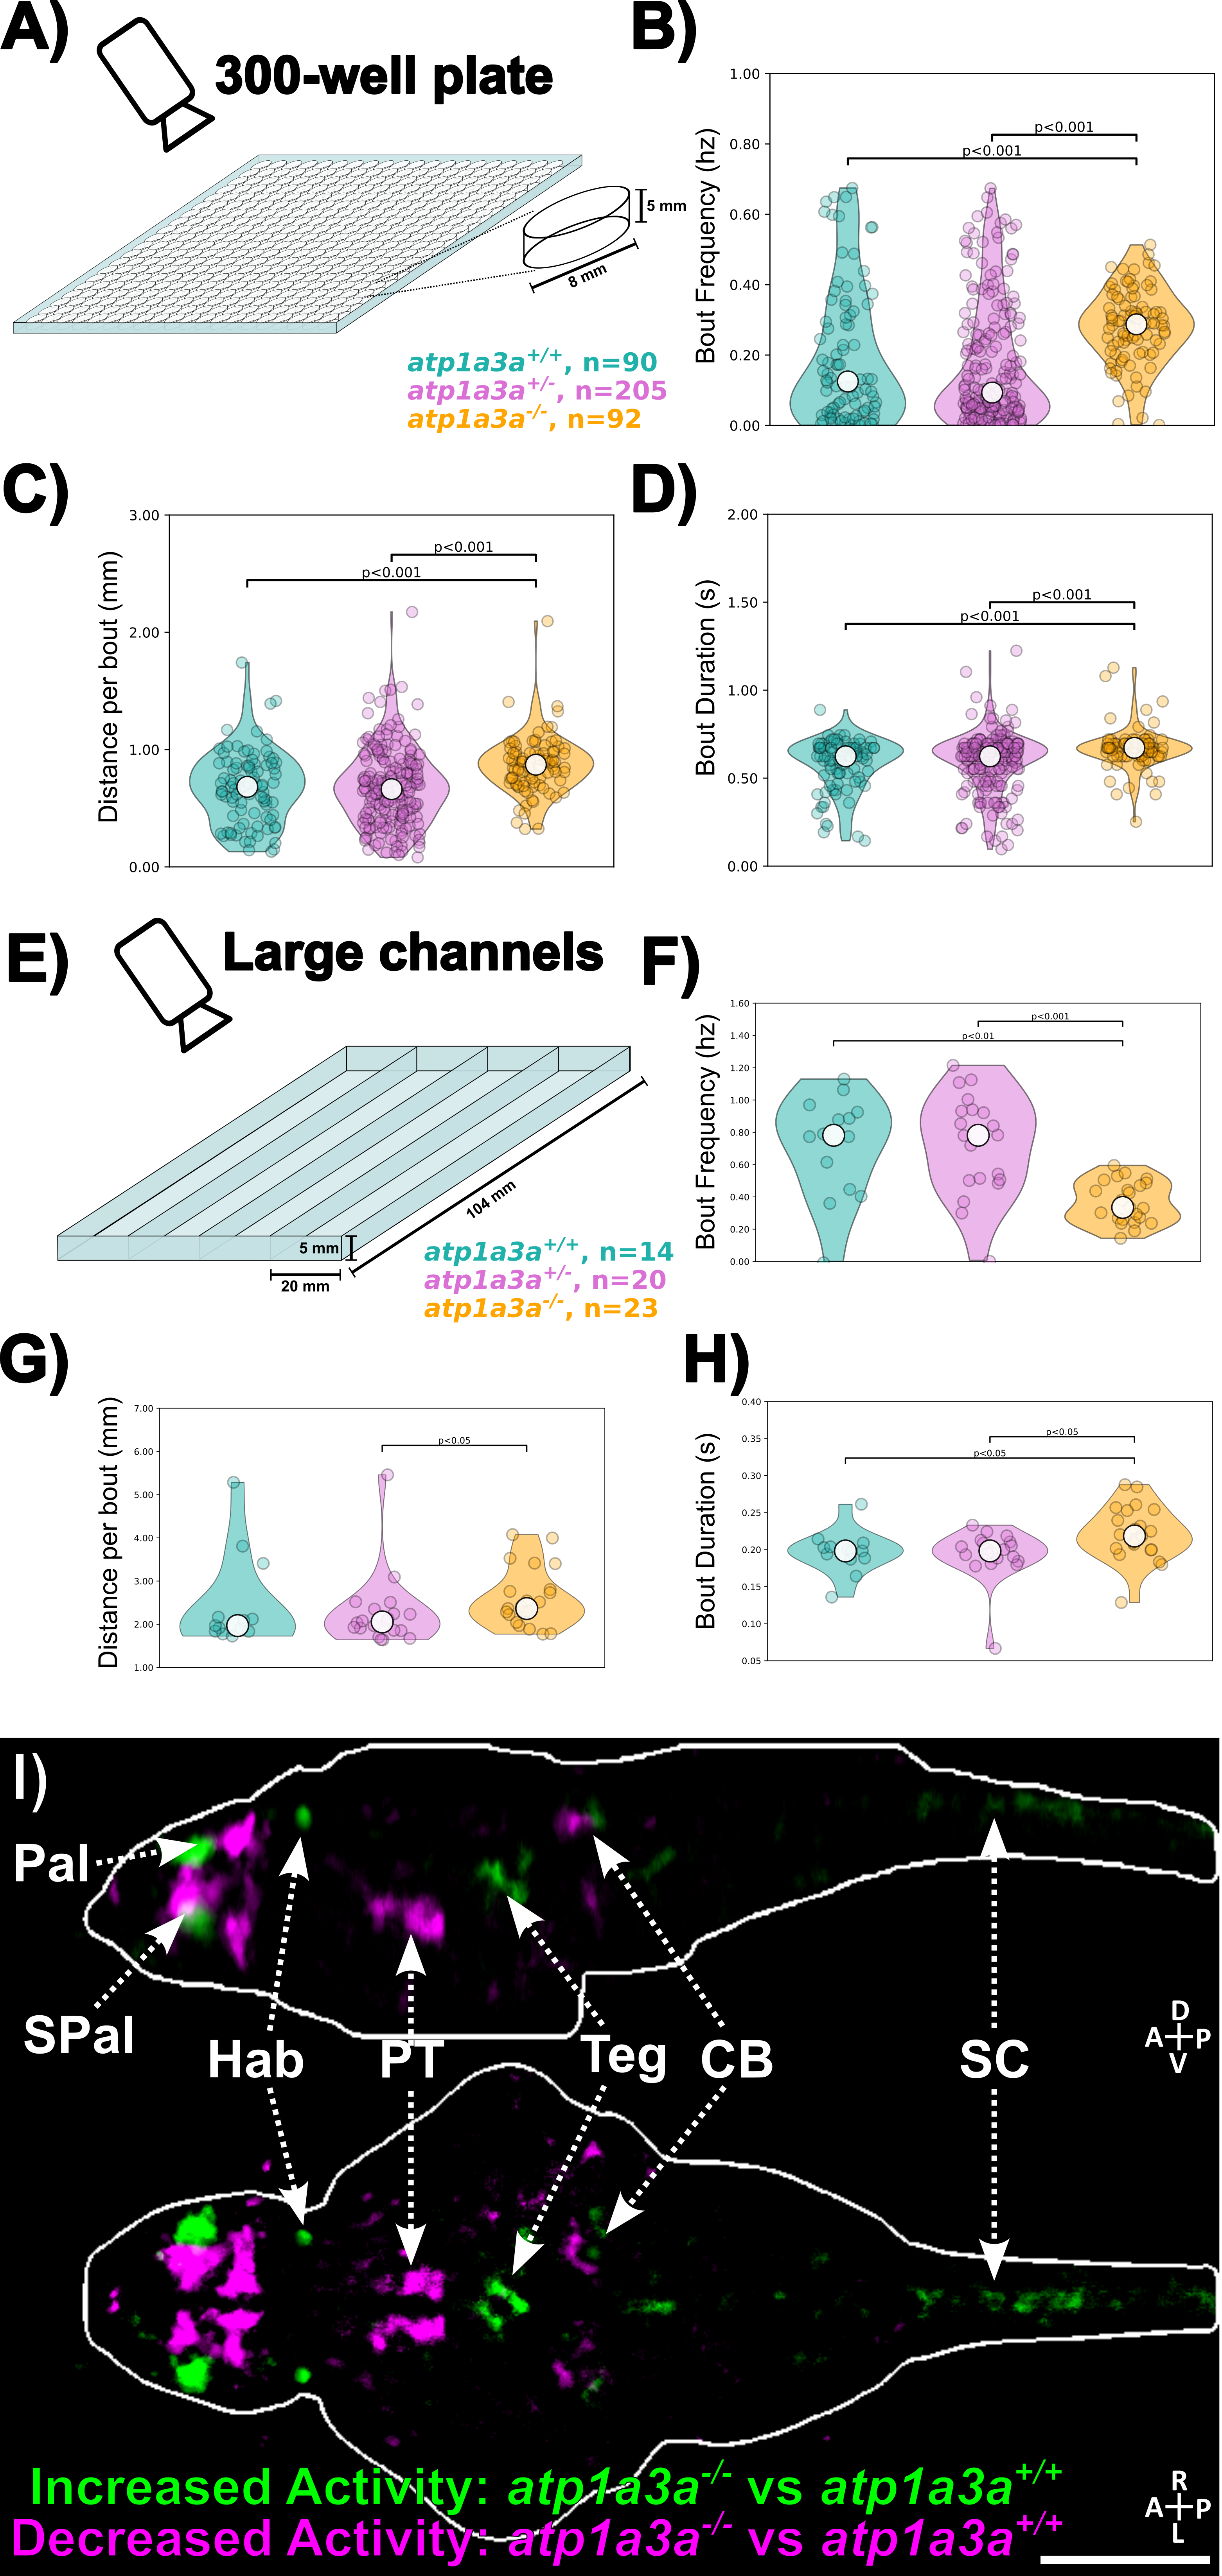
\includegraphics[width=0.9\linewidth]{Figures/Figure_FreeSwimming.png}

\caption{\textbf{\emph{atp1a3a} mutants are hyperactive under spontaneous conditions, and show altered activity patterns concentrated in the forebrain}\\
Analysis of spontaneous swimming behaviour in 300-well plates \citep{Lamire2023-he} over a 30 min recording period revealed that \emph{atp1a3a} mutants show significantly increased: 
\textbf{A)} total displacement, 
\textbf{B)} movement bout initiation frequency, 
\textbf{C)} displacement per bout, and
\textbf{D)} duration of bouts. 
Statistics: Kruskal-Wallis with Dunn's multiple comparisons test.
\\ \textbf{E)} MAP-Mapping analysis of brain-wide activity patterns in \emph{atp1a3a} mutants relative to WT siblings revealed a distributed but fairly restricted pattern of altered activity, with strong activation and suppression patterns in the forebrain, including the pallium (Pal), subpallium (SPal), habenula (Hab), and diencephalon in the posterior tuberculum (PT) and preoptic area. 
More modest changes are seen in the cerebellum (CB) spinal cord (SC) and midbrain tegmentum (TEG). 
Scale bar = 100 \textmu m.
}

\label{fig:2}
\end{center}
\end{figure}

Having established that \emph{atp1a3a} mutants exhibit complex behavioural abnormalities via qualitative observation, we sought to more systematically characterize their phenotypes under spontaneous conditions, and to identify potential underlying neural circuit dysfunctions. For this purpose, we observed larvae in a multi-well setup under normal lighting conditions, in which 300 larvae can be observed simultaneously. \citep{Randlett2019-fj,Lamire2023-he}. 
Consistent with previous results \citep{Barlow2023}, we found that \emph{atp1a3a\textsuperscript{-/-}} larvae display hyperactivity, characterized by increased total displacement, increased bout frequency, increased median displacement per bout and increased median bout duration (\autoref{fig:2}D-E). 
Therefore, mutants are hyperactive and not only initiate more movement bouts, but also move in larger bouts. 
Under these conditions, we did not observe significant phenotypes in heterozygous \emph{atp1a3a\textsuperscript{+/-}} larvae, indicating that such gross movement phenotypes may be more specific to the homozygous condition, or that the heterozygous condition has more subtle, transient, or less penetrant phenotypes that are not revealed by these population-wide analyses.

In order to identify potential neural substrates and brain areas involved in these abnormal swimming phenotypes, we mapped the brain-wide activity of \emph{atp1a3a} mutants relative to their WT siblings using the MAP-Mapping approach \citep{Randlett2015}. 
MAP-Mapping uses immunostaining of phospohylated ERK (pERK) relative to total-ERK (tERK) levels as a proxy for neuronal activity, combined with image volume registration and statistical analysis to identify regions with altered pERK/tERK ratios, and presumably altered neuronal activity.
We analyzed cohorts of larvae that were left to swim freely in a 10cm petri dish in a brightly lit environment, and determined group genotyping post-imaging. 
pERK/tERK ratios were compared voxel-wise to generate a brain-wide statistical map of altered activity under these baseline behavioural conditions (\autoref{fig:2}E).

Based on the widespread expression of \emph{atp1a3a} in the brain, as well as the very strong and broad electrophysiological phenotypes expressed in other ATP1A3-deficient models, we expected to see very widespread alterations in neural activity across many brain areas.
In contrast, MAP-Mapping revealed a distributed but fairly restricted pattern (\autoref{fig:2}E). 
Consistent with the hyperactivity or perhaps dysregulated motor coordination in these mutants, we saw significant activation in some motor-areas, including the spinal cord and midbrain tegmentum, while the cerebellum showed areas of both increased and decreased activity.
Much more prominent alterations in pERK/tERK signals were seen in the forebrain, including the pallium, subpallium and habenula. 
The potential relationships with these altered forebrain activity patterns and hyperactivity is not clear, but do indicate that these areas of the brain appear to be particularly sensitive to \emph{atp1a3a} loss, and thus may be critical for understanding the circuit-level mechanisms underlying the behavioural phenotypes in these mutants. 

\subsection{Behavioural and neural phenotypes in \emph{atp1a3a} mutants in stimulus-evoked conditions}

\begin{figure}
\begin{center}
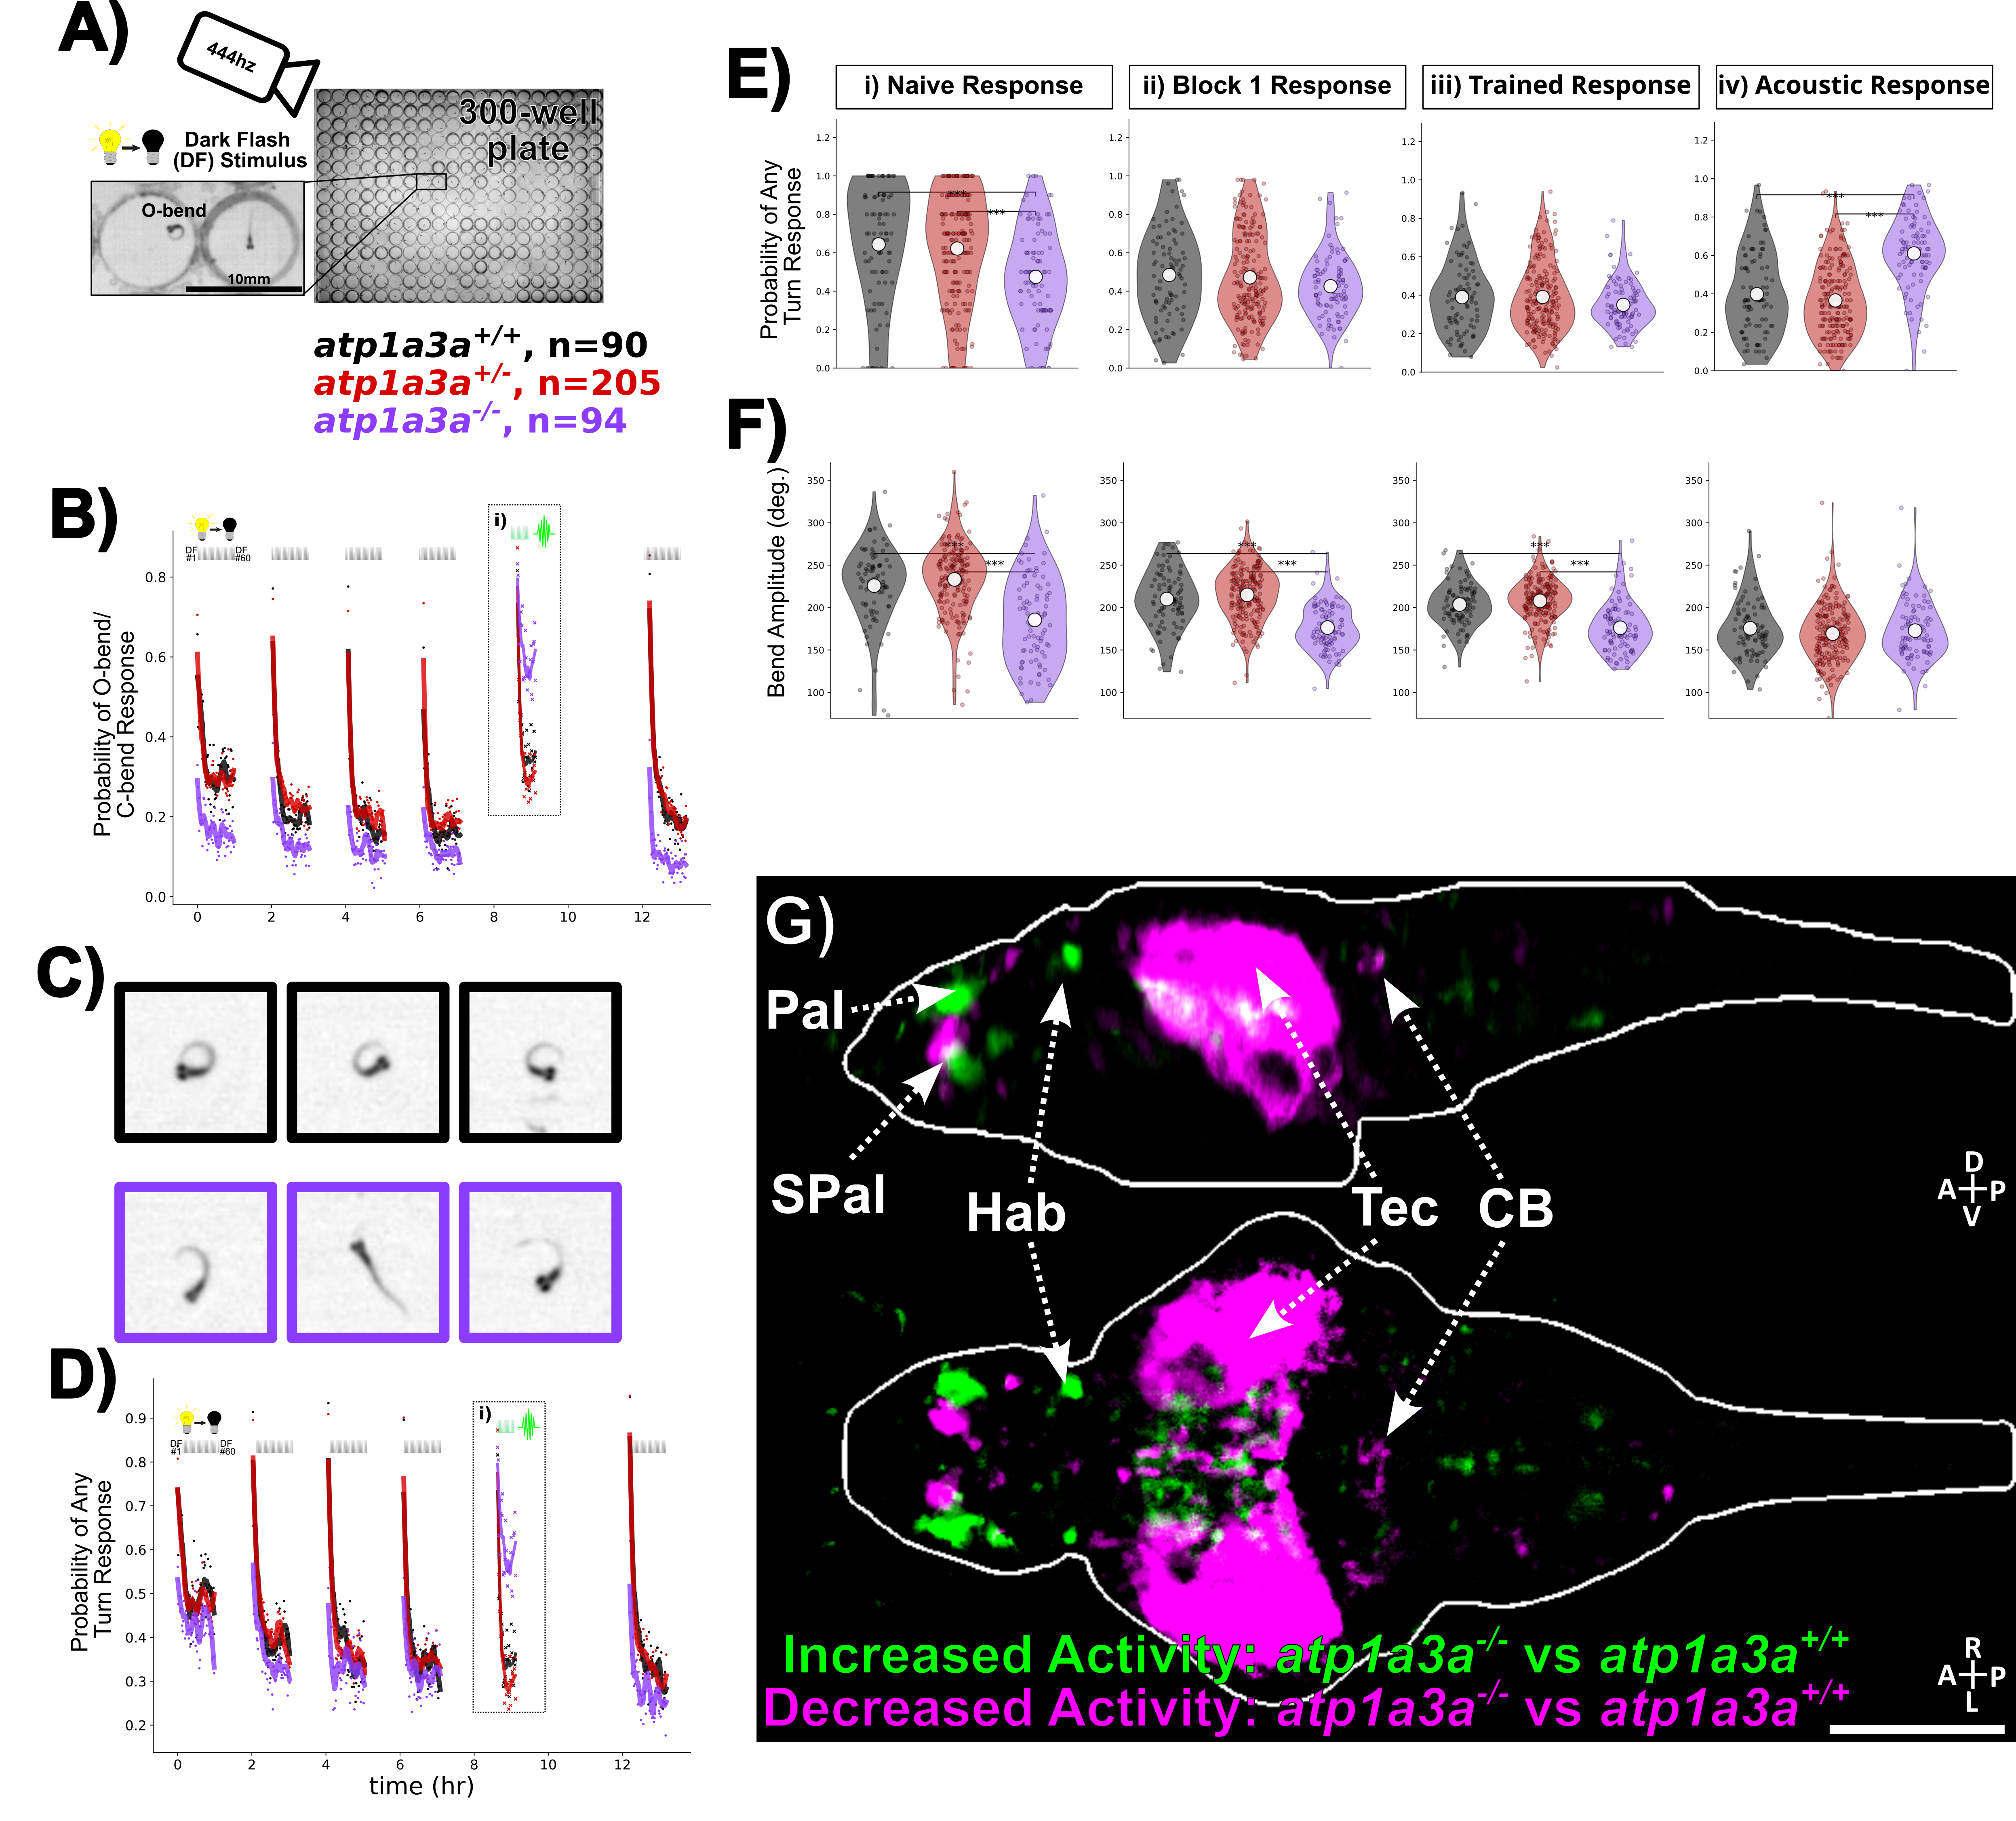
\includegraphics[width=0.9\linewidth]{Figures/Figure_DarkFlash.png}


\caption{\textbf{\emph{atp1a3a} mutants show reduced behavioural responses to Dark Flash stimuli and altered neuronal activation in the midbrain and forebrain}\\
\textbf{A)} Multiwell setup for quantifying responses to Dark Flash (DF) stimuli, in which 300 larvae can be observed simultaneously. \citep{Randlett2019-fj, Lamire2023-he}.
\\ \textbf{B)} Response curves comparing \emph{atp1a3a} mutants to heterozygous and WT siblings, showing a reduced response across 5 blocks of 60 DF stimuli delivered at 1 min intervals. 
Boxed area \textbf{(i)}, shows the response to 30 acoustic/"tap" stimuli, delivered at 1min intervals, for which mutants show an exaggerated response relative to siblings.
Dots represent mean population response probability for each stimulus, and lines are smoothed across time/stimuli with a Savitzky–Golay filter (window = 15 stimuli, order = 2). O-bend responses to DF and C-bend responses to tap stimuli are defined as turns with a bend amplitude of at least 3 radian, and 1 radian, respectively.
\\ \textbf{C)} Examples of the maximal bending amplitude of three WT (black) and mutant (purple) larvae in response to a dark flash, showing the reduced response amplitude in mutants.  
\\ \textbf{D)} Same data as \textbf{(B)}, but analyzed to consider any turning response, defined as a bend of at least 1 radian, which reveals a more similar response probability between mutants and siblings, suggesting that mutants are able to respond to the stimulus, but with reduced amplitude.
\\ \textbf{E)} Per-fish quantification of the probability of turning responses, and \textbf{F} quantification of the maximal bend amplitude in response to stimuli, for different epochs of the experiment: \textbf{i)} the Naive Response to the first 5 DFs, \textbf{ii)} the remainder of the first training block (DFs 6-60), \textbf{iii)} the trained response in blocks 2-4 (DFs 61-240), and \textbf{iv)} the response to tap stimuli (Taps 1-30). Significance tests are Kruskal-Wallis tests with Dunn's multiple comparisons test, * p < 0.05, ** p < 0.01, *** p < 0.001.
\\ \textbf{E)} MAP-Mapping analysis of brain-wide activity patterns in \emph{atp1a3a} mutants relative to WT siblings after being stimulated with 10 DFs at 1min intervals. The signals in the optic tectum (Tec) are stronlgy suppressed, while the cerebellum (CB) and hindbrain areas show more modest alterations. 
Strong activation and suppression patterns are seen in the forebrain, including the pallium (Pal), subpallium (SPal), habenula (Hab).
Scale bar = 100 \textmu m.
}

\label{fig:3}
\end{center}
\end{figure}


To test the stimulus-response behaviour of \emph{atp1a3a} mutants, we began with our standard 300-well screening assay (\autoref{fig:3}A), in which larvae are exposed to trains of "Dark Flash" stimuli (DF, a sudden transition to darkness that initiates the O-bend response), and acoustic/tap stimuli (a brief vibrational stimulus delivered with a solenoid rod that initiates the C-bend response) \citep{Burgess2007-2}. 
Stimuli are delivered at 1 minute intervals, and the response probability and kinematics are quantified for each stimulus across the population of larvae.
This revealed that \emph{atp1a3a} mutants show a very strongly reduced probability of executing an O-bend response to the DFs, indicating that they may be mostly blind to this stimulus (\autoref{fig:3}B). 
However, visual analyses of the responses to DFs revealed that many mutants did appear to respond, but did so with a reduced amplitude of bending, which does not meet our criteria for an "O-bend" response, defined as a turn with a minimal bend amplitude of 3 radian (\autoref{fig:3}C, \citealp{Randlett2019-fj}).
When we relaxed these criteria to consider any turning response within the 1-second of the DF stimulus, we found that the response probability of mutants was much more similar to siblings (\autoref{fig:3}D), demonstrating that mutants are mostly still able to respond to the stimulus, and only show a significantly reduced probability of responding in the initial phase of the assay (\autoref{fig:3}Ei-iii), but do so with a strongly reduced bending amplitude (\autoref{fig:3}Fi-iii).
This may either reflect a reduced ability to execute large amplitude bends, or perhaps that the perceived strength of the stimulus is reduced in mutants, leading to a reduced motor response.


To gain insight into the neural substrates underlying the reduced responses to DFs, we performed MAP-Mapping analysis of brain-wide activity patterns in \emph{atp1a3a} mutants relative to WT siblings after being stimulated with 10 DFs at 1 min intervals ()\autoref{fig:3}G).
This revealed a very strong suppression of activity in the optic tectum, which is the largest primary visual area in the zebrafish brain, and shows strong responses to DFs in WT larvae \citep{Lamire2023-he}. This indicates that the visual DF response is suppressed early in the visual pathway, suggesting sensory deficits early in the circuit. 
Suppressed responses were also observed in the cerebellum, and similar to what we observed in the spontaneous condition, we saw relatively subtle alterations in hindbrain areas. Again, the most striking alterations were seen in the forebrain, including the pallium, subpallium and habenula, which show strong patterns of both activation and suppression relative to WT siblings (\autoref{fig:3}G).

In contrast to the reduced responses to DFs, \emph{atp1a3a} mutants showed an increased response probability to acoustic/tap stimuli (\autoref{fig:3}Bi, Di, Eiv), with a bend amplitude indistinguishable from controls (\autoref{fig:3}Fiv). 
Therefore, \emph{atp1a3a} mutants are not simple hyporesponsive to stimuli, but exhibit very different effects in different assays, indicating a differential role for Atp1a3a in different circuit contexts. 


\begin{figure}
\begin{center}
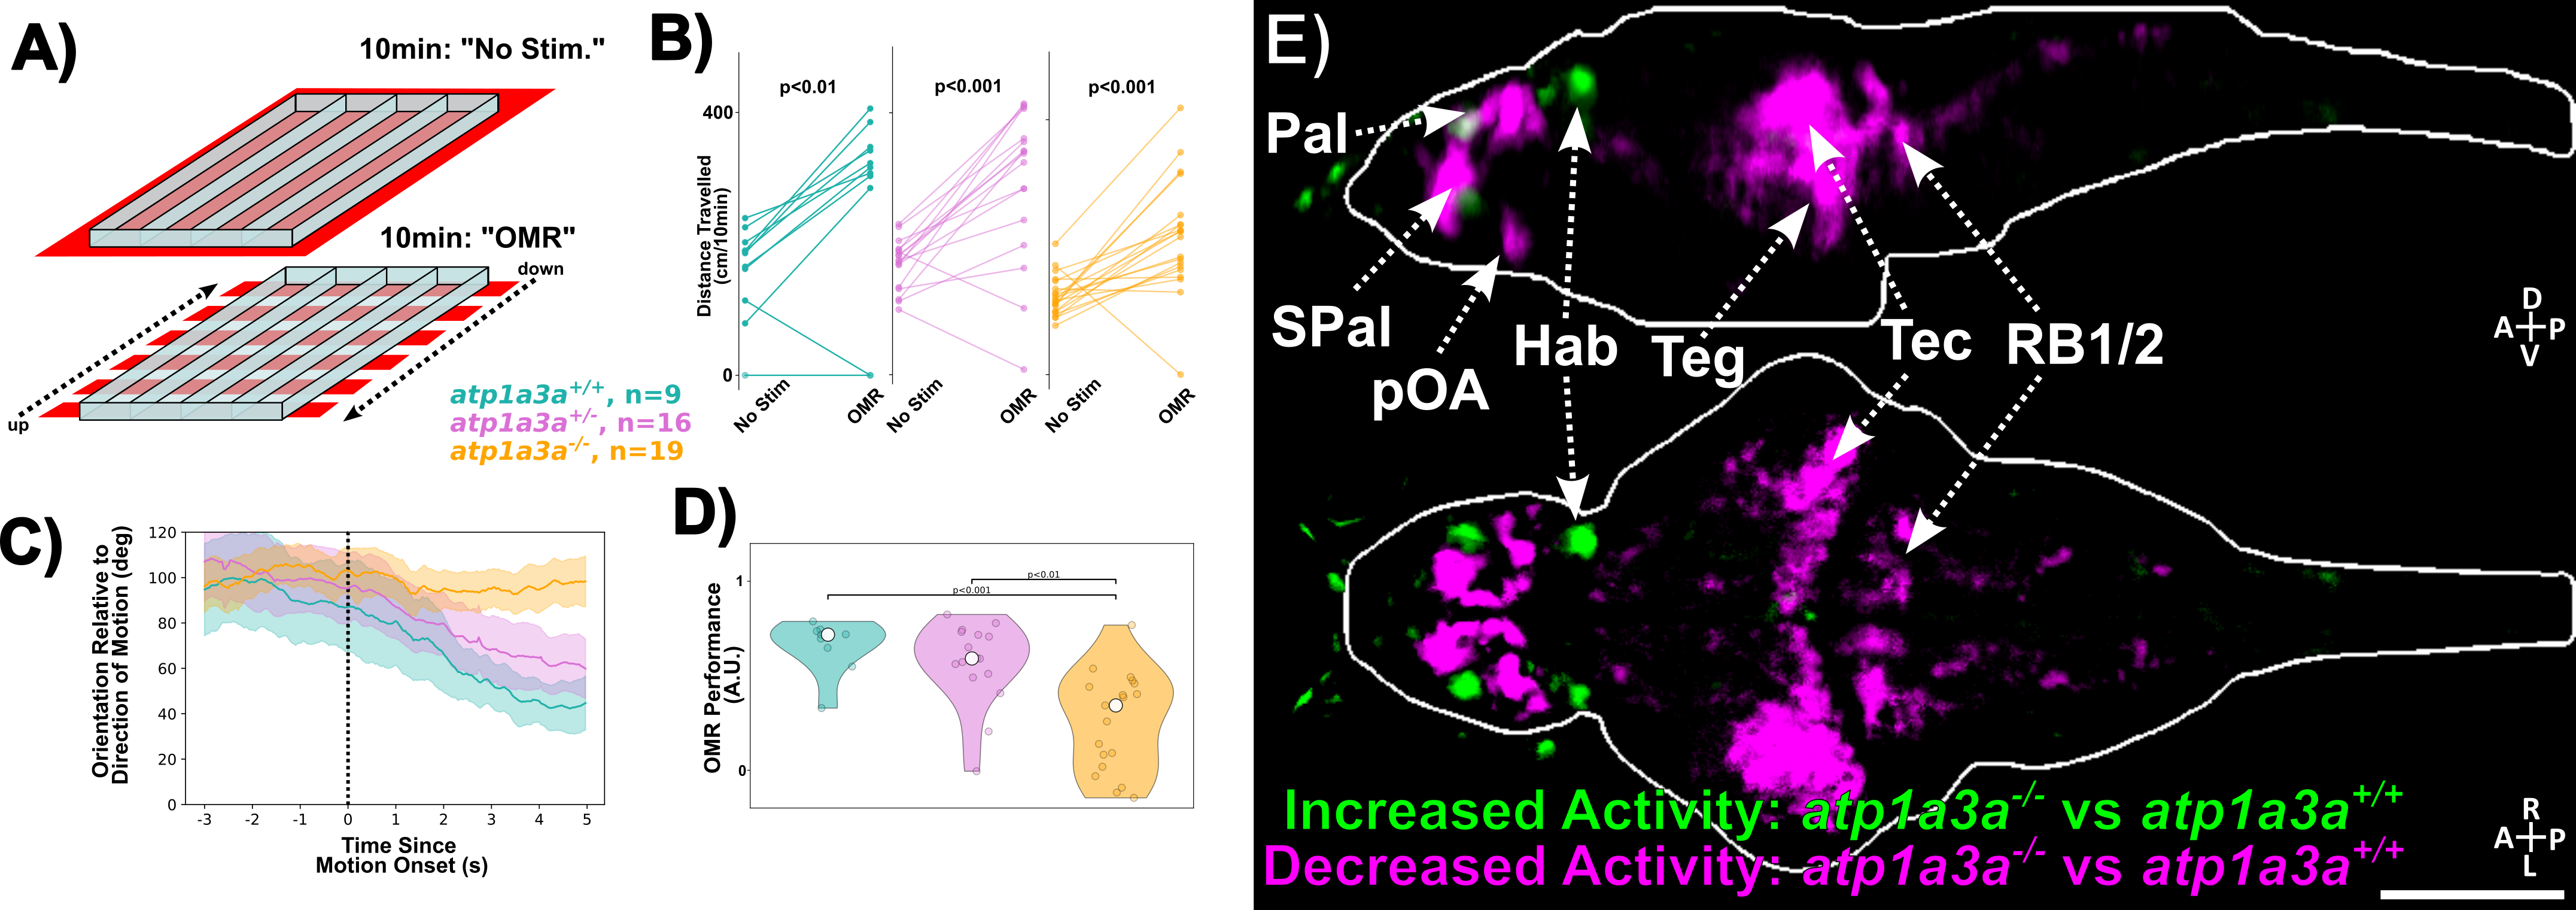
\includegraphics[width=0.9 \linewidth]{Figures/Figure_OMR.png}


\caption{\textbf{\emph{atp1a3a} mutants show reduced directional responses to Optomotor stimuli and altered neuronal activation in the midbrain and forebrain}\\
\textbf{A)} Arena for Optomotor Response (OMR) assay, in which larvae are placed in tracks and either presented with global red light for the stimulus-free condition ("No Stim."), or with moving striped patterns that elicit robust directional swimming responses in WT larvae ("OMR Stim.").
\textbf{B)} \emph{atp1a3a} mutants and siblings show a robust increase in swimming during the OMR stimulus, indicating that they are able to perceive the stimulus and respond with increased swimming activity.
\textbf{C)} \emph{atp1a3a} mutant larvae show a significantly reduced turning response to the direction of motion, with a much smaller realignment of the orientation of the larvae towards the axis of motion of the stimulus (0 degrees would reflect perfect alignment). Lines = mean orientation across larvae, shaded area = SEM.
\textbf{D)} \emph{atp1a3a} mutants show a reduced ratio of vertical swimming relative to horizontal swimming, indicating a reduced ability to use the motion cues to guide their swimming direction.
\textbf{E)} MAP-Mapping analysis of brain-wide activity patterns in \emph{atp1a3a} mutants relative to WT siblings after being stimulated with the OMR stimulus. Similar to the DF stimulus, we observed a strong suppression of activity in the midbrain optic tectum (Tec) and tegmentum (Teg). Suppressed activity is also seen in the anterior hindbrain Rhomboemeres 1 and 2 (RB1/2). Strong activation and suppression patterns are again seen in the forebrain, including the pallium (Pal), subpallium (SPal), habenula (Hab) and preoptic area (pOA).
}

\label{fig:4}
\end{center}
\end{figure}

The optomotor response is an intensively studied visuomotor behaviour in which larvae respond to whole-field moving stimuli with robust directional swimming responses \citep{Portugues2009}. 
To test the optomotor response in \emph{atp1a3a} mutants, we placed larvae in an arena in which they can swim freely in rectangular channels while being presented with either global red light (No-Stimulus condition) or a striped pattern moving along the tracks alternating between upwards and downwards motion (OMR condition) (\autoref{fig:4}A). 
We quantified the response of larvae to this motion in three ways: 
1) increased swimming  (\autoref{fig:4}B), 
2) turning towards the direction of motion, which is visible as a realignment of the mean orientation of the larvae towards the axis of stimulus motion within a few seconds of motion onset (\autoref{fig:4}C),
3) proportionately increased swimming of the fish in the vertical dimension (following motion cues), relative to horizontal dimension (orthogonal to motion cues) (\autoref{fig:4}D).
Interestingly, \emph{atp1a3a} mutant larvae showed a robust increase in swimming during the stimulation period, indicating that they are able to perceive the stimulus and respond with increased swimming activity (\autoref{fig:4}B). 
However, they showed a significantly reduced turning response to the direction of motion, with a much smaller realignment of the orientation of the larvae towards the axis of motion of the stimulus (\autoref{fig:4}C). 
Mutants also showed a reduced increase in vertical swimming relative to horizontal swimming (\autoref{fig:4}D), indicating a reduced ability to use the motion cues to guide their swimming direction.
We note also that mutants showed hypoactivity relative to WT siblings in the "No-Stimulus" condition (\autoref{fig:4}B, p=0.049, Kruskal-Wallis/Dunn's), indicating that there is a context dependence to the hyperactivity phenotype in mutants that we observed in our multi-well assay (\autoref{fig:2}A). The hypoactivity observed here is related to the different lighting, larger arena, or differing handling during the experiment (see Methods).

We again then used this OMR assay to perform MAP-Mapping analysis of brain-wide activity patterns in \emph{atp1a3a} mutants relative to WT siblings after being stimulated with the OMR stimulus (\autoref{fig:4}E).
Similar to the DF stimulus (\autopageref{fig:3}G), we observed a strong suppression of activity in the optic tectum -- though in a clearly distinct more posterior/ventral pattern, likely reflecting the differential topographic presentation of the OMR stimulus below the animals. 
We observed relatively little change in the diencephalic pretecum, which is thought to be more critical than the tectum for motion processing in the context of the OMR \citep{Matsuda2021-a, Wang2020-a}, indicating that this area may be less affected in \emph{atp1a3a} mutants.
However, activity was strongly suppressed in multiple ares of the anterior hindbrain (Rhombomeres 1/2), which has been associated with OMR sensorimotor processing \citep{Chen2018-sdf}, as well as turn direction regulation through the ARTR \citep{Dunn2016-asd}. 
Therefore, the reduced OMR turning responses in \emph{atp1a3a} mutants may be related to dysfunction in these areas. 
Similar to the DF stimulus, we observed strong patterns of both activation and suppression in the forebrain, including the pallium, subpallium and habenula, again consistent with a model in which these areas are particularly sensitive to \emph{atp1a3a} loss ireespective of stimlus or behavioural context.  


\subsection{\emph{atp1a3a} mutants show dysregulated activity in the forebrain and basal-ganglia related circuitry across different stimulus and behavioural contexts}

\begin{figure}
\begin{center}
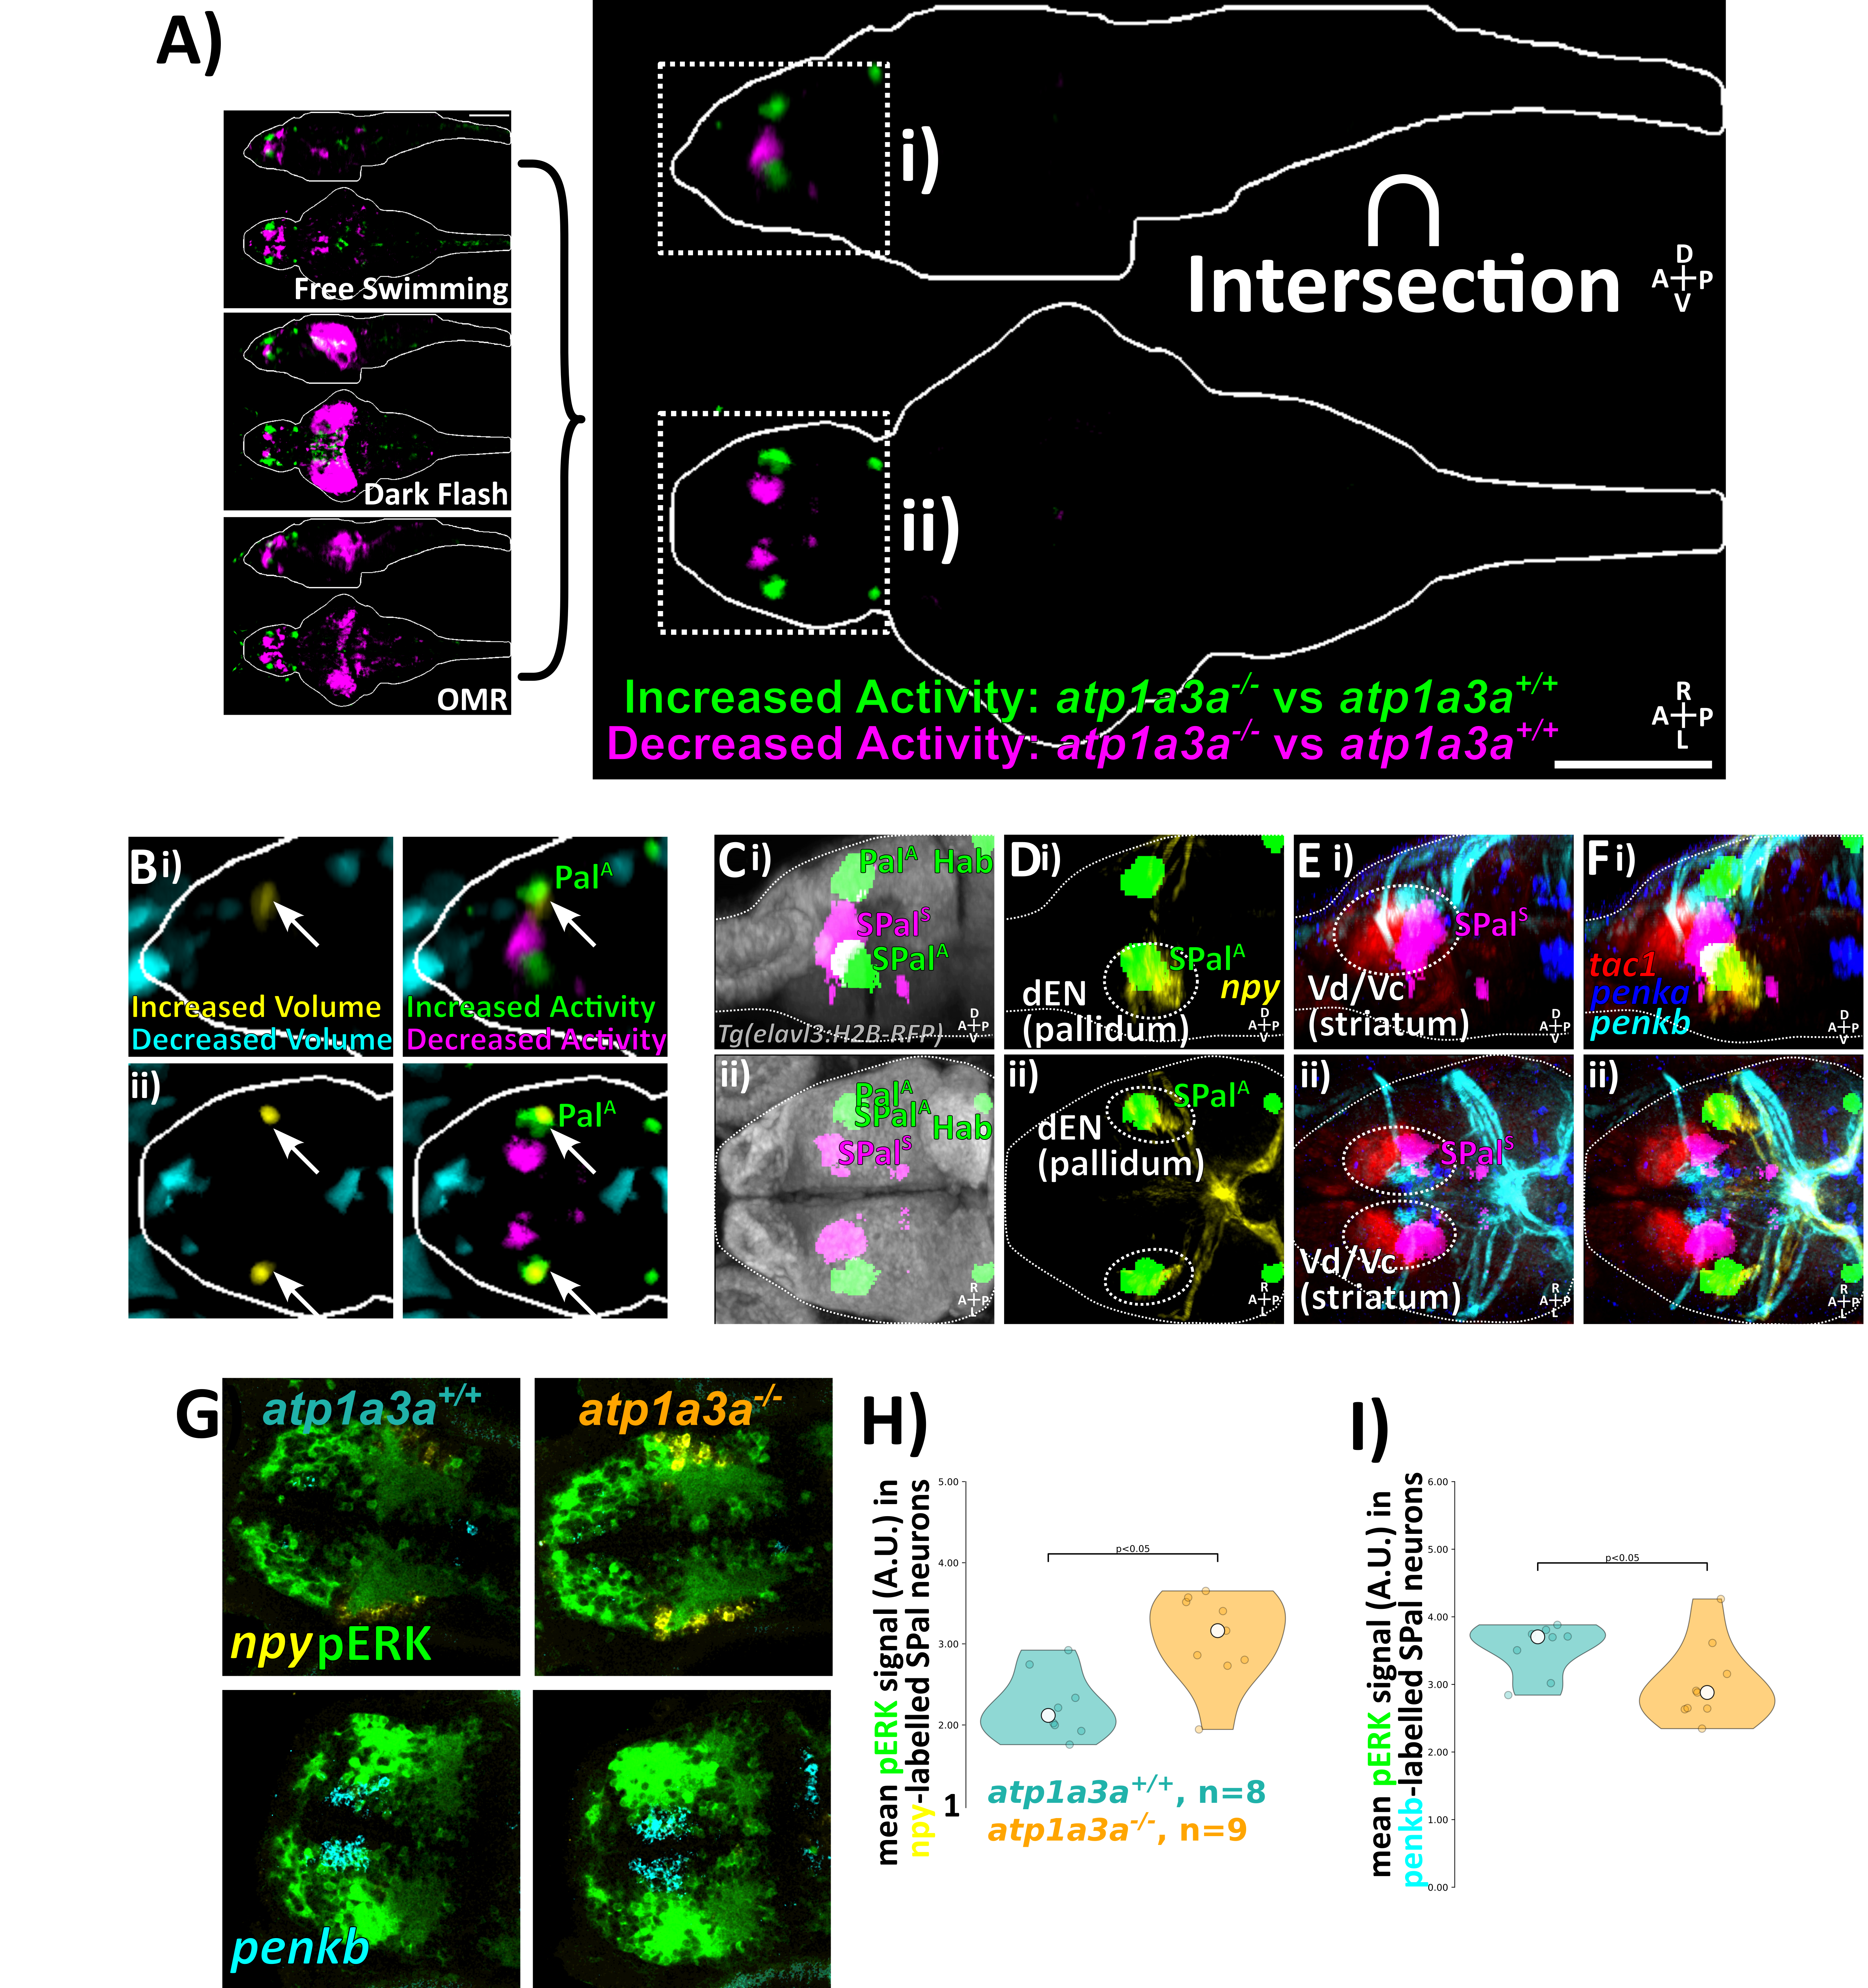
\includegraphics[width=0.6 \linewidth]{Figures/Figure_Intersection.png}


\caption{\textbf{Dysregulated activity in the forebrain of \emph{atp1a3a} mutants in the habenula and areas homologous to the basal ganglia}\\
\textbf{A)} Arena for Optomotor Response (OMR) assay, in which larvae are placed in tracks and either presented with global red light for the stimulus-free condition ("No Stim."), or with moving striped patterns that elicit robust directional swimming responses in WT larvae ("OMR Stim.").
\textbf{B)} Activity patterns displayed on top of the Z-Brain atlas marker for neuronal nuclei (\emph{Tg(elavl3:H2B-RFP)}) \citep{Randlett2015} for the telencephalic region in \textbf{i)} saggital,  \textbf{ii)} dorsal projections. Activivation is seen in the Habneula (HB\textsuperscript{A}), lateral pallium (Pa\textsuperscript{A}), and subpallium (SPa\textsuperscript{A}), while suppression is seen in the more medial subpallium (SPa\textsuperscript{S}).
\textbf{C)} Activation patterns shown relative to the \emph{npy} (yellow), highlighting the colocalization of this dEN (pallidum) marker with (SP\textsuperscript{A}). 
\textbf{D)} Suppression patterns shown relative to the \emph{tac1} (red), \emph{penka} (blue) and \emph{penkb} (cyan), highlighting the proximity of these Vd/Vc (striatum) markers with (SPa\textsuperscript{S}).
\textbf{E)} Overlap of all markers and activity patterns
}


\label{fig:5}

\videosupp{Rotating 3D projection of common telencepahalic activity patterns in \emph{atp1a3a} mutants relative to basal ganglia markers. Same color scheme as \autoref{fig:5}B-E. 
Download: \href{\detokenize{https://raw.githubusercontent.com/owenrandlett/2025_atp1a3a/main/Manuscript/Figures/Supplements/SupplementaryMovie_RotatingProjectionTelencephalon.mp4}}{SupplementaryMovie\_RotatingProjectionTelencephalon.mp4}
\label{videosupp:basalganglia1}}
\end{center}
\end{figure}



Our behavioural and neural imaging experiments revealed that \emph{atp1a3a} mutants show dramatic behavioural alterations across various different contexts, including postural problems, hyper- and hypo-activity, reduced responses to visual stimuli, and increased responses to acoustic/tap stimuli. 
Based on this limited sampling of behavioural phenotypes, it is difficult to determine how these different phenotypes may relate to one another, and whether they are related to dysfunction in the same or different brain areas and circuits.
In our MAP-Mapping experiments focusing on three stimulus contexts (No stimulus, Dark Flashes and OMR), we observed some expected altered activity patterns in known areas, such as the optic tectum and hindbrain, that could explain some of the stimulus-specific phenotypes.
However, some of the most dramatic patterns were in the forebrain, and appeared to be highly consistent across experiments: including the pallium, subpallium and habenula. 

To examine the consistencies in these patterns quantitatively, we directly compared the MAP-Mapping results across these three experiments by generating an intersection map, where only pixels that show significant alterations in all three experiments are retained (\autoref{fig:5}A).
This revealed a very striking and bilaterally symmetrical pattern of altered activity, with a zone of co-activation in the habenula (HB\textsuperscript{A}), activation of the lateral pallium (Pa\textsuperscript{A}), and two zones of activation and suppression in the subpallium (SP\textsuperscript{A} and SP\textsuperscript{S}, respectively). 

The zebrafish habenula is thought to functions as a key integrative hub linking sensory inputs and internal state to downstream neuromodulatory circuits, thereby regulating aversive processing, stress coping, attention, and action selection \citep{Okamoto2021}. 
Distinct dorsal and ventral habenular subdivisions contribute differentially to these processes, with the dorsal habenula modulating innate and state-dependent behaviors and the ventral habenula supporting associative learning.
Therefore, altered habenular activity in \emph{atp1a3a} mutants may contribute to the altered stimulus responses and hyperactivity phenotypes through dysregulated sensory processing.

The pallium and subpallium are the major divisions of the telencephalon, where the pallium is homologous to the mammalian cortex and contains predominatntly excitatory neuronal populations, while the subpallium comprises conserved telencephalic domains homologous to the mammalian basal ganglia, septal nuclei, and components of the extended amygdala, giving rise predominantly to inhibitory neuronal populations involved in action selection, motivation, and emotional processing \citep{Wullimann2004}.
Dystonia and other ATP1A3-related neurological disorders are widely thought to arise, at least in part, from dysfunction within basal ganglia circuits, which play a central role in motor control, action selection, and the regulation of movement vigor \citep{Brggemann2021}. 
We were therefore particularly interested in examining basal ganglia–associated structures to assess whether the altered subpallial activity is occurring within these conserved motor circuits.

Tanimoto et al., have recently defined markers for the basal ganglia homologs in zebrafish based on conserved gene expression and connectivity analyses \citep{Tanimoto2024}, which we used to operationally define the larval zebrafish basal ganglia subregions in our activity maps. 
In this framework, \emph{tac1} and \emph{penkb} are used as markers of Vd/Vc, the homologs of the striatum, while \emph{npy} and \emph{nkx2.1} demarcate the dorsal entopeduncular nucleus (dEN), the homolog of pallidum. 
We stained for \emph{tac1}, \emph{penka}, \emph{penkb} and \emph{npy} using HCR in situ hybridization, and registered these images to the Z-Brain atlas \citep{Randlett2015} (\autoref{fig:5}B-E, \autoref{videosupp:basalganglia1}).
This revealed that the zone of suppressed activity in the subpallium (SP\textsuperscript{S}) overlaps with the Vd/Vc striatal homologs, while the zone of activated activity (SP\textsuperscript{A}) overlaps with the dEN homolog (\autoref{fig:5}B).
This pattern of striatial suppression and pallidal activation is consistent with the known inhibitory connectivity among these regions, and is consistent with a model in which basal ganglia circuits may be particularly sensitive to ATP1A3-loss. 

\subsection{Ca2\textsuperscript{2+} imaging identifies altered sensorimotor responses and abnormal bursting activity in the \emph{atp1a3a} mutant forebrain}


\begin{figure}
\begin{center}
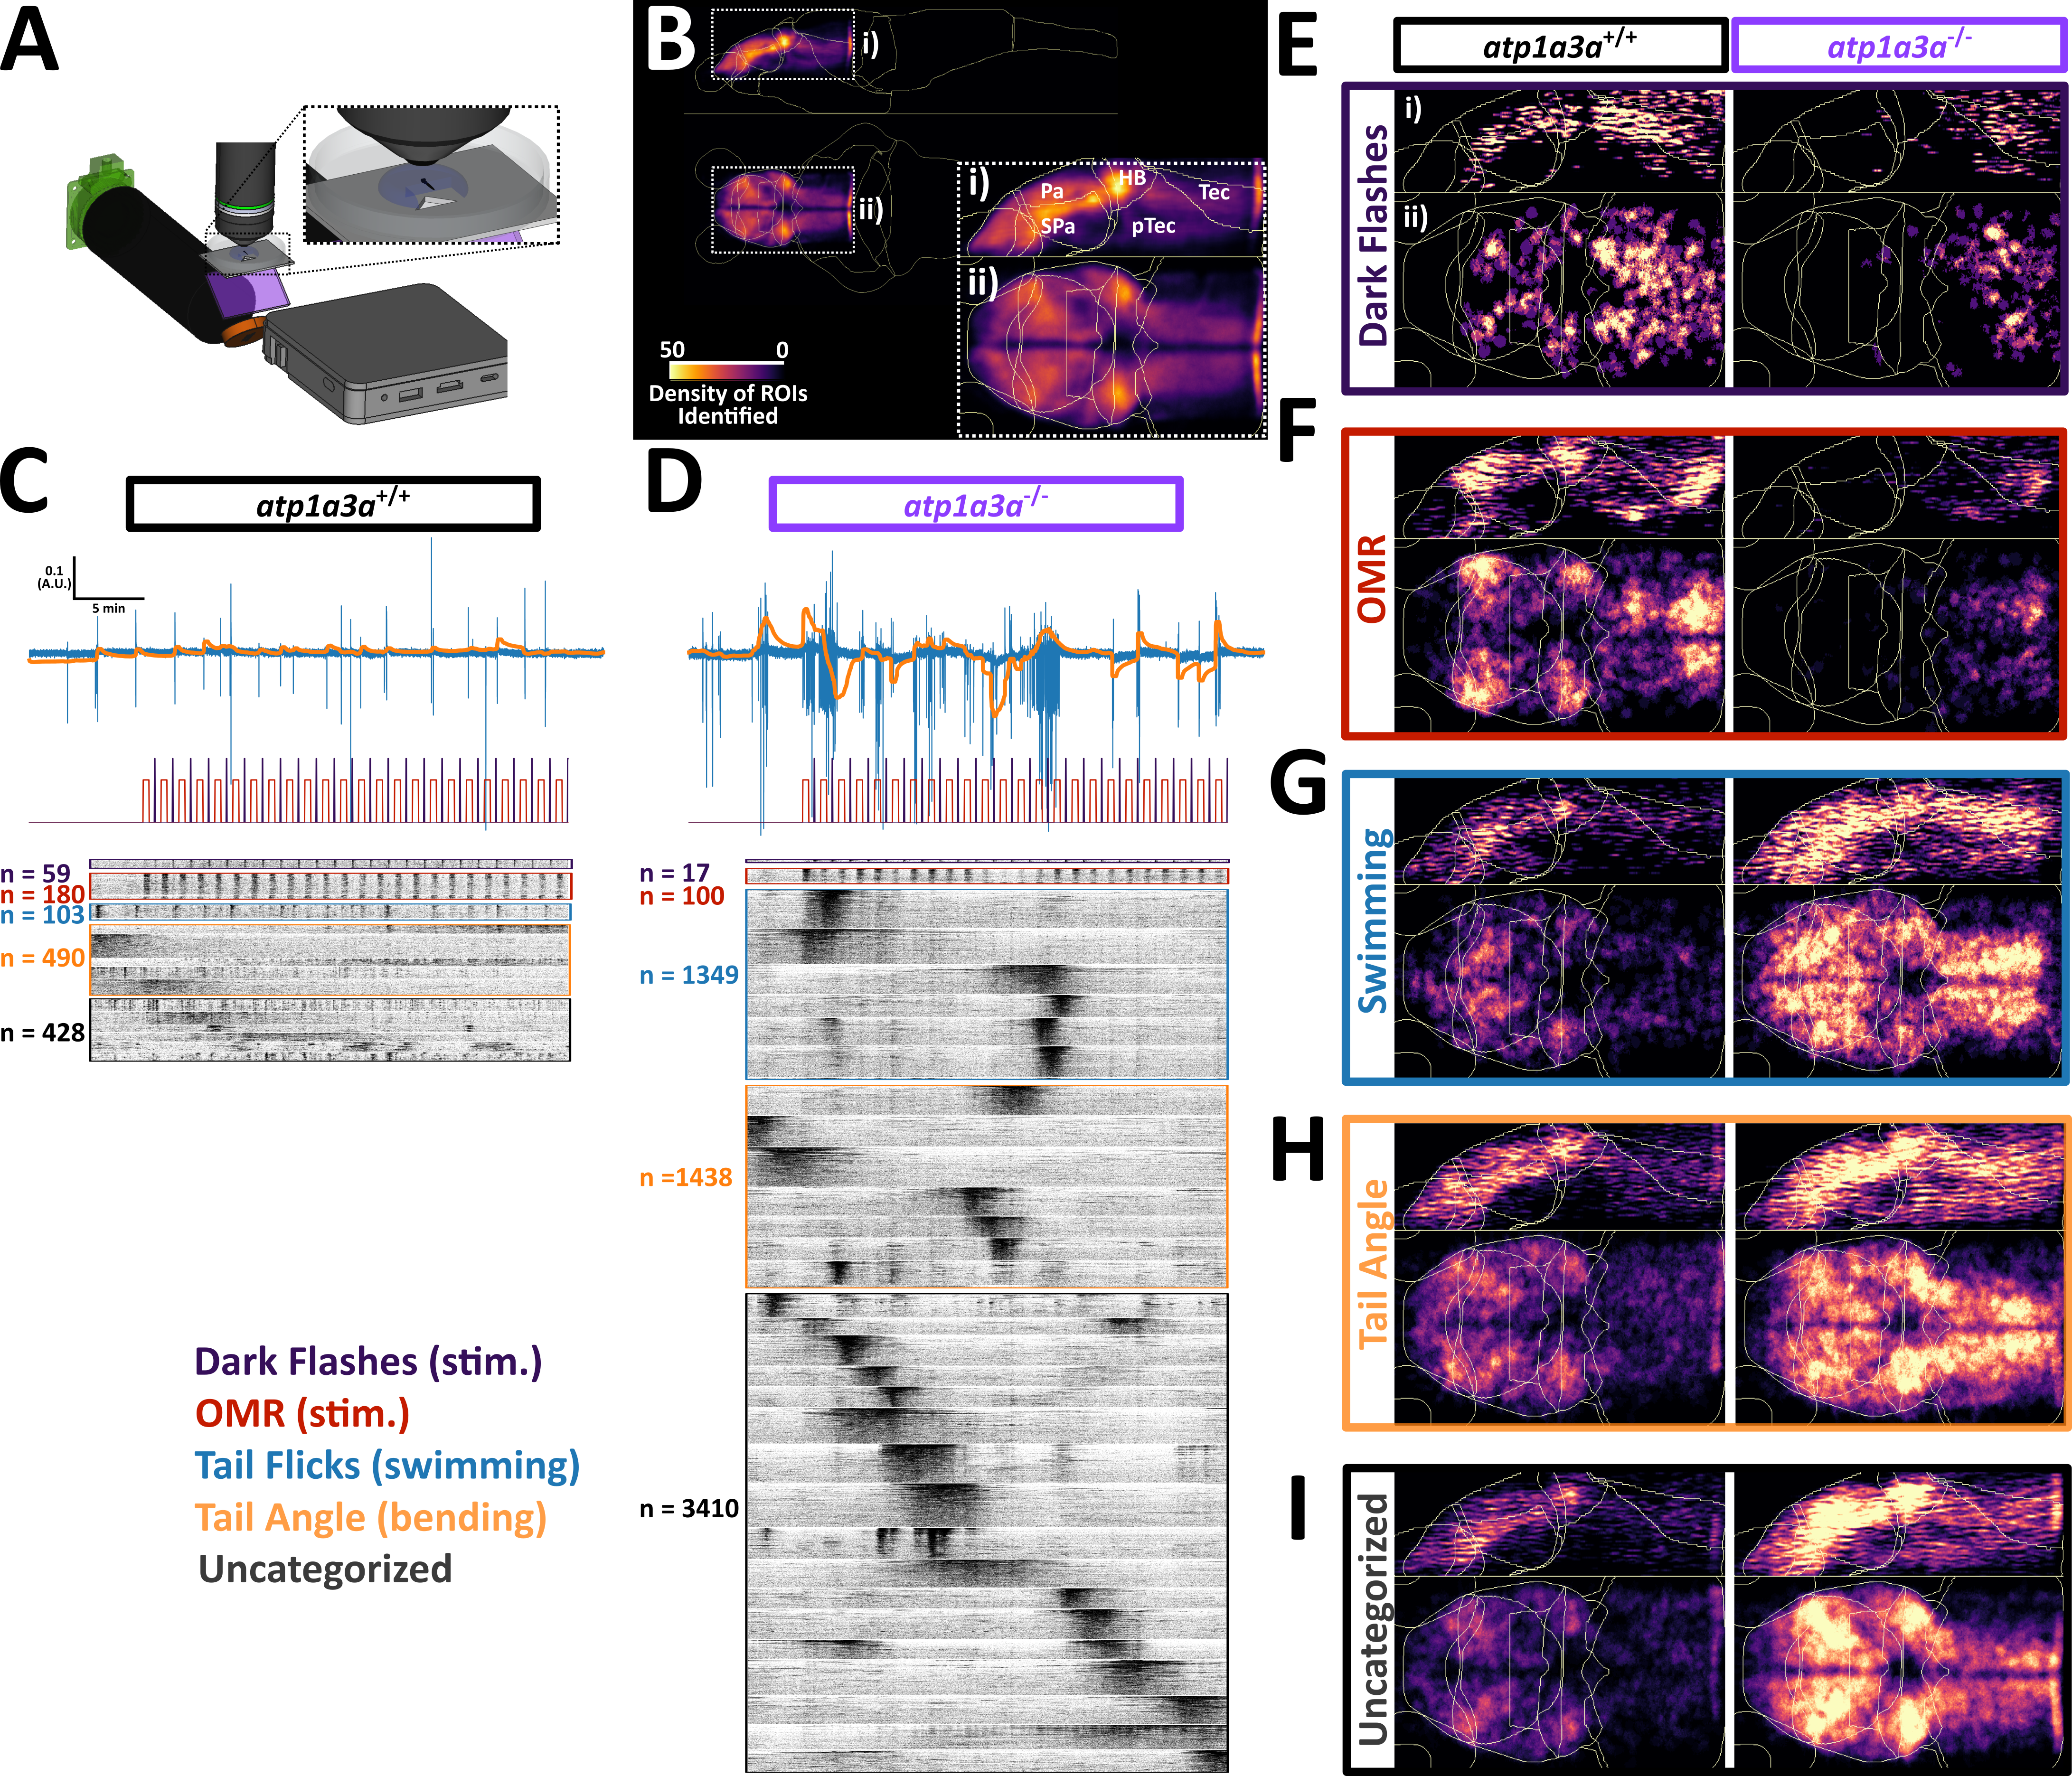
\includegraphics[width=0.9 \linewidth]{Figures/Figure_Ca2Imaging.png}


\caption{\textbf{Ca\textsuperscript{2+} imaging of \emph{atp1a3a} mutant forebrain activity}\\
\textbf{A)} asdfadfasdf
}


\label{fig:6}


\figsupp[Regional quantification of identified neurons across genotypes.]
{Regional quantification of identified neurons across genotypes..
\textbf{A)} 
}{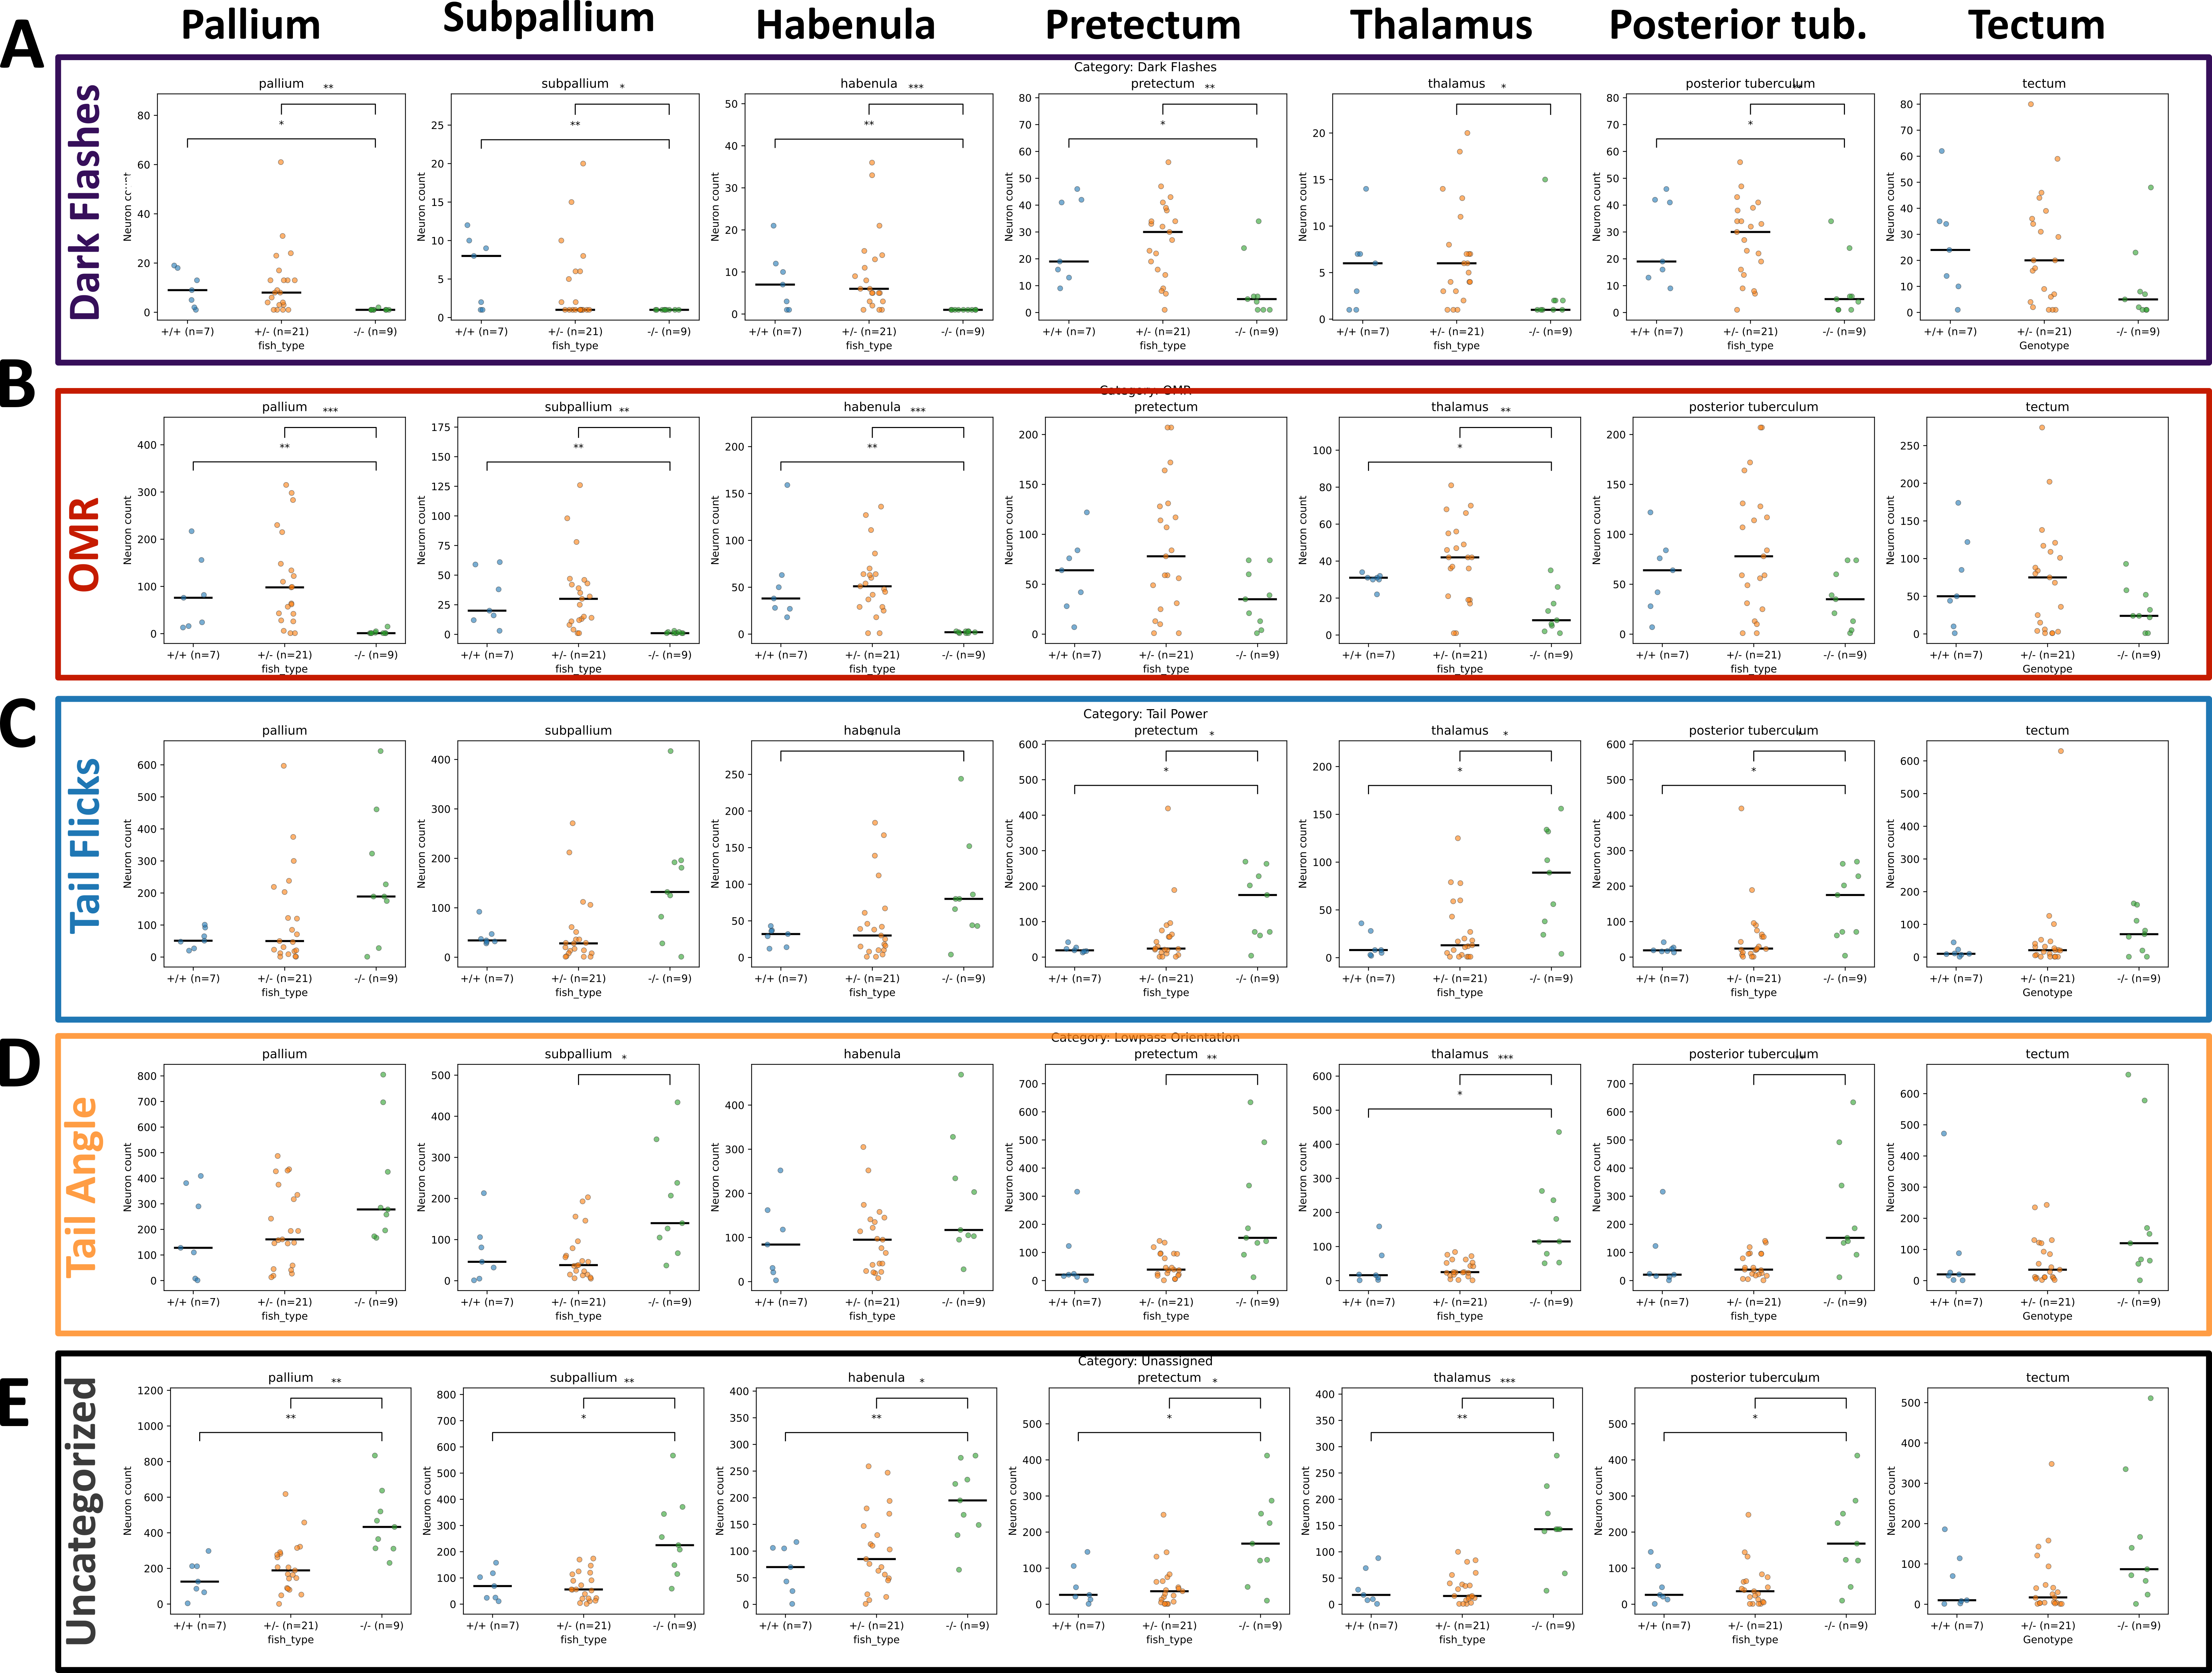
\includegraphics[width=0.9\linewidth]{Figures/SupplementartFig_RegionQuantification_Ca2Imaging.png}}
\label{fig:S6}

\figsupp[Activity heatmaps of \emph{atp1a3a} mutants, compared to heterozygous and wild-type siblings.]
{Activity heatmaps of \emph{atp1a3a} mutants, compared to heterozygous and wild-type siblings.
\textbf{A)}
<<<<<<< HEAD
}{\includegraphics[width=0.9\linewidth]{Figures/SupplementartFig_Ca2Heatmaps.png}}
=======
}{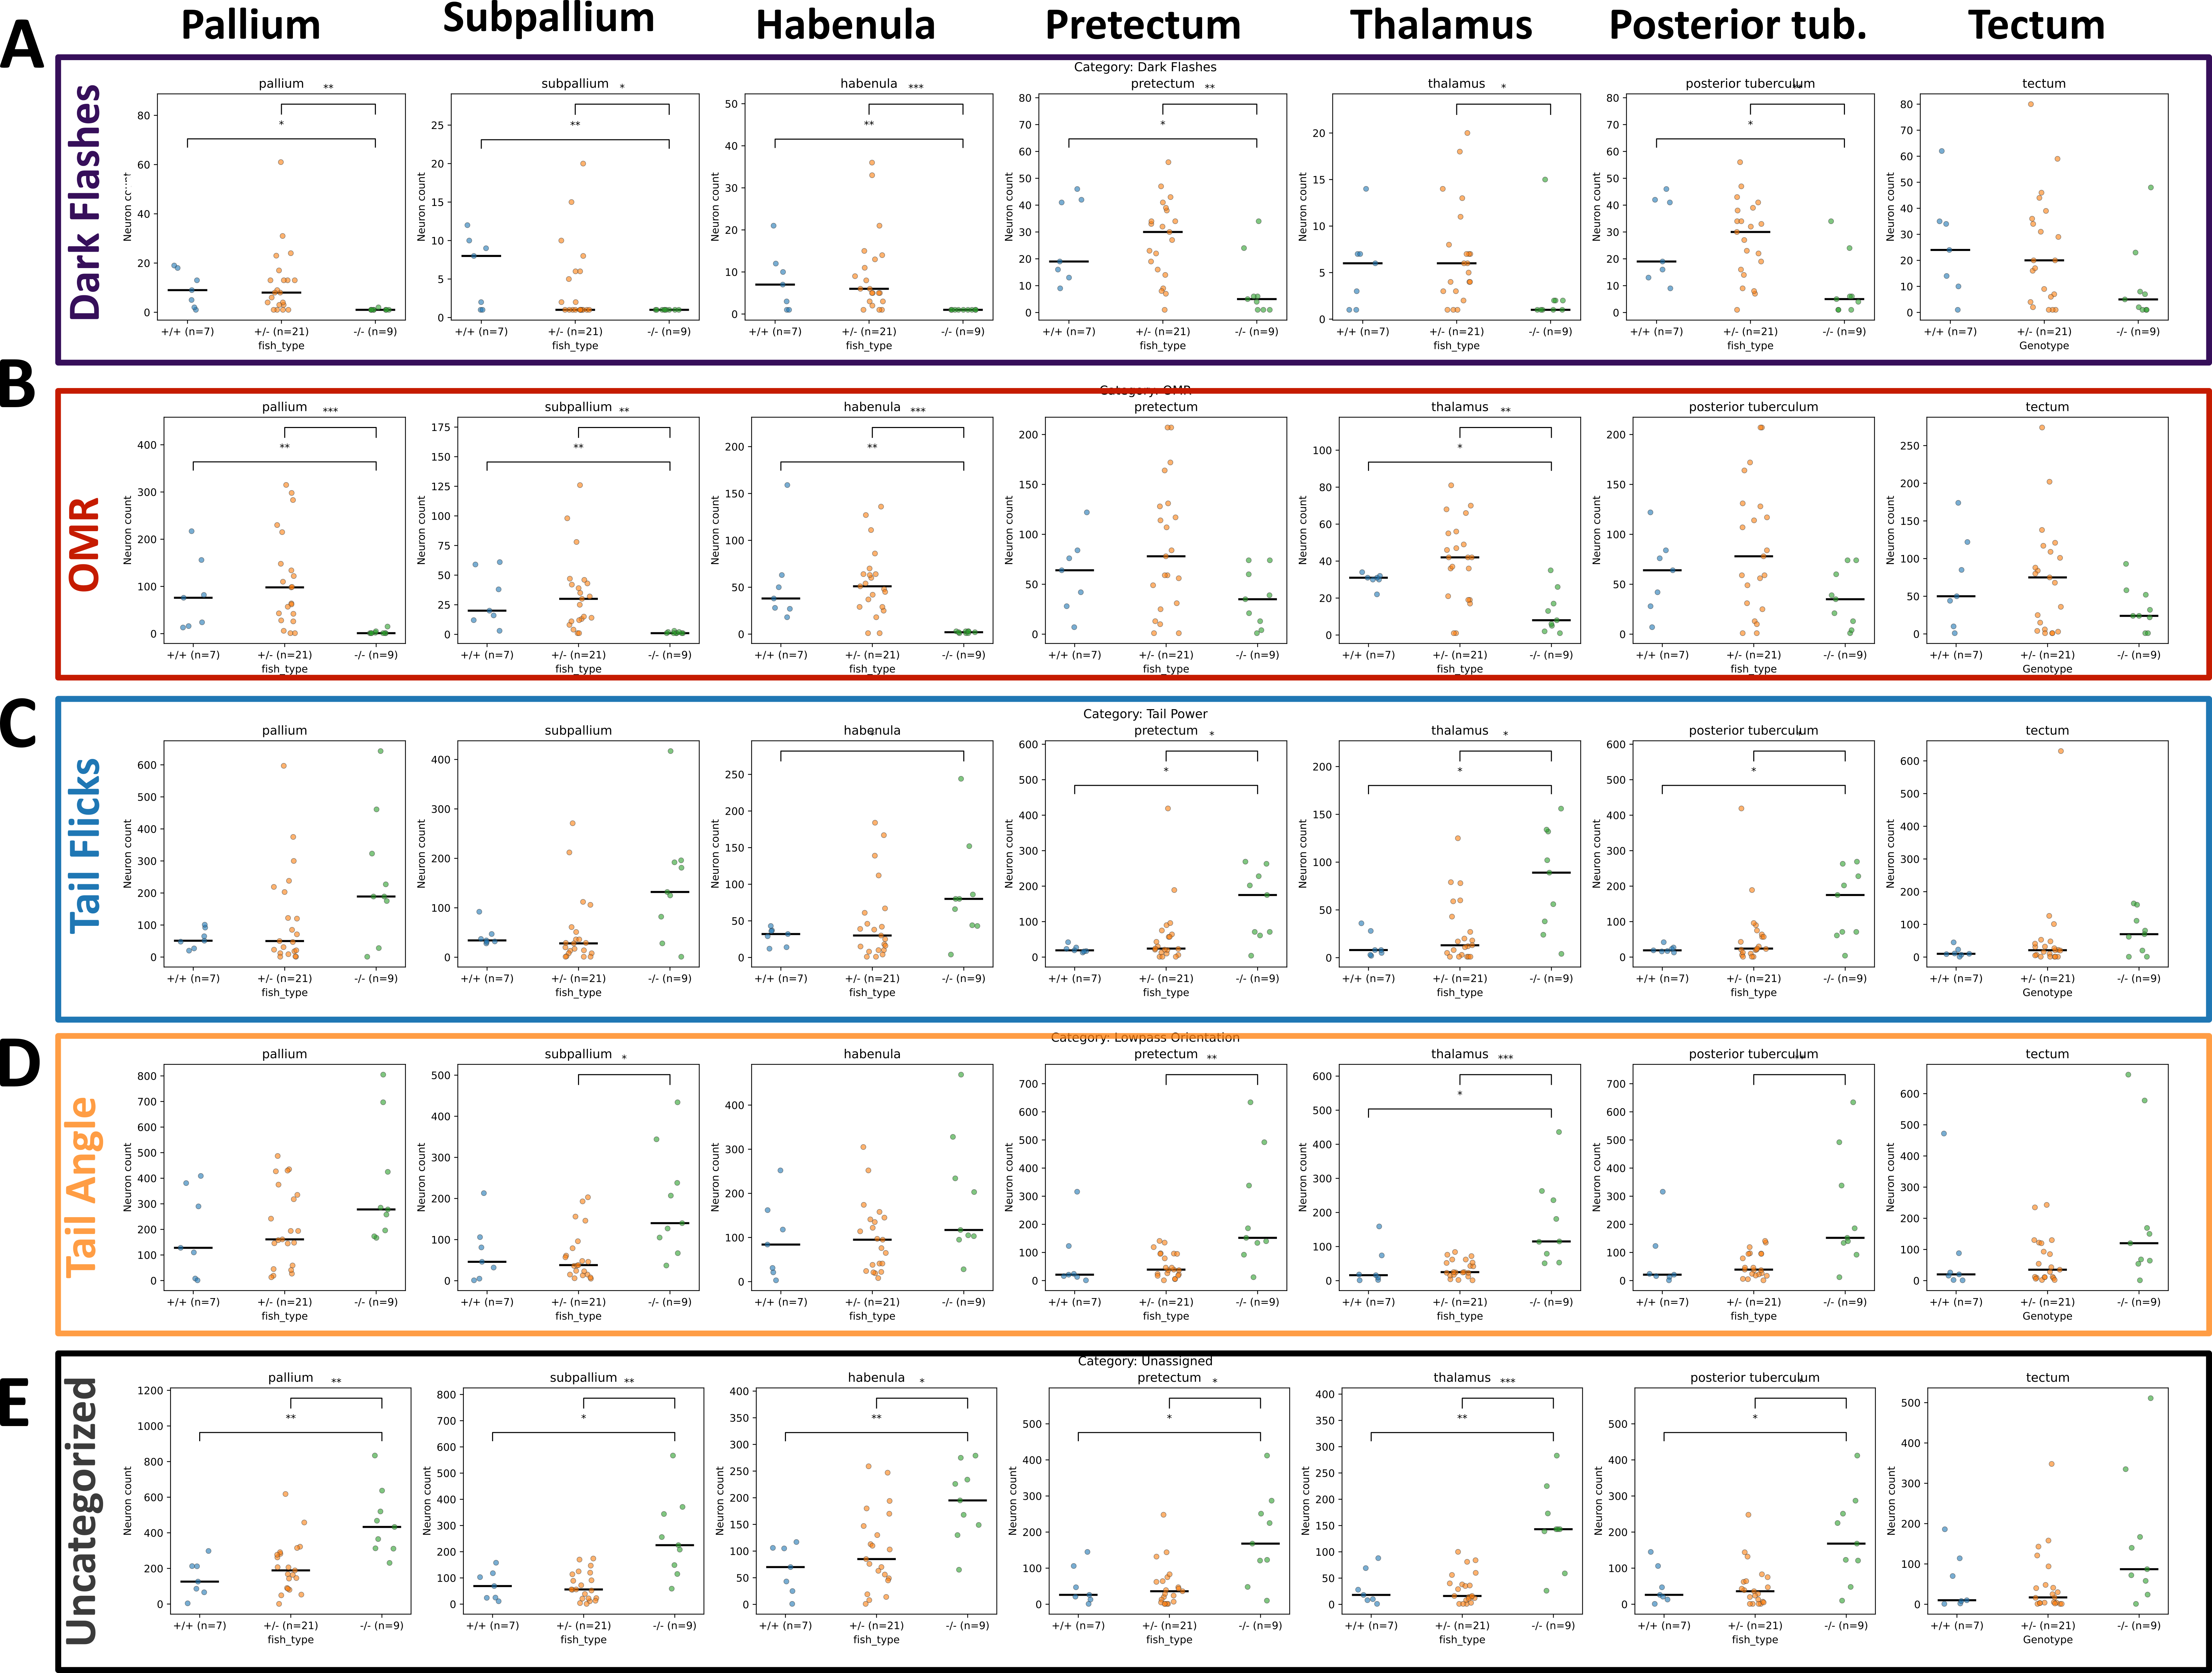
\includegraphics[width=0.9\linewidth]{Figures/SupplementartFig_RegionQuantification_Ca2Imaging.png}}
>>>>>>> bdfdd3b3e2c66e1ab9786d2a5998a762c0aa5a56
\label{fig:S6b}

\end{center}
\end{figure}
\vspace{3mm}

While pERK is a very useful proxy for neuronal activity, it is an indirect measure that reflects the integrated activity of neurons over a timescale of minutes, and thus does not capture the fast dynamics of neural activity that are critical for sensorimotor processing.
<<<<<<< HEAD
To gain insight into the fast dynamics of neural activity in \emph{atp1a3a} mutants, we performed volumetric 2-photon Ca\textsuperscript{2+} imaging of the forebrain.
We crossed \emph{atp1a3a} mutants with a transgenic line that expresses the nuclear-targeted GCaMP6f Ca\textsuperscript{2+} indicator pan-neuronally, in the pigment deficient \emph{Nacre} mutants (\emph{Tg(elavl3:H2B-GCaMP6f); mitfa\textsuperscript{-/-}}), to generate a line that allows for brain-wide Ca\textsuperscript{2+} imaging in \emph{atp1a3a}. 

Larvae were imaged while head-embedded in agarose with the tail free to move and imaged with a modified \emph{pi\_tailtrack} apparatus \citep{Randlett2023}, integrating a video projector in order to present dynamic visual stimuli onto a screen below the larvae (\autoref{fig:6}A). Larvae were imaged over a 15-minute period, in a volume covering the areas of the forebrain showing the consistent altered activity patterns observed using pERK (\autoref{fig:5}, \autoref{fig:6}B). 
Larvae were presented with alternating DFs and 10 second pulses of forward OMR motion, repeated at 30 second intervals. 
This allowed us to compare how these stimuli are represented in forebrain neurons in the mutant brain, which we have established generate differential behavioural responses and pERK-derived activity patterns (\autoref{fig:2,fig:3,fig:4}). 
=======
To gain insight into the fast dynamics of neural activity in \emph{atp1a3a} mutants, we performed volumetric 2-photon Ca\textsuperscript{2+} imaging of the forebrain in response to sensory stimuli.
We crossed \emph{atp1a3a} mutants with a transgenic line that expresses the nuclear-targeted GCaMP6f Ca\textsuperscript{2+} indicator pan-neuronally, in the pigment deficient \emph{Nacre} mutants (\emph{Tg(elavl3:H2B-GCaMP6f); mitfa\textsuperscript{-/-}}), to generate a line that allows for brain-wide Ca\textsuperscript{2+} imaging in \emph{atp1a3a}. 

Larvae were imaged while head-embedded in agarose with the tail free to move and imaged with a modified \emph{pi\_tailtrack} apparatus \citep{Randlett2023}, integrating a video projector in order to present dynamic visual stimuli onto a screen below the larvae (\autoref{fig:6}A). Larvae were imaged over a 15-minute period, in a volume covering the areas of the forebrain showing the consistent altered activity patterns observed using pERK (\autoref{fig:5}, \autoref{fig:6}B). 
Larvae were presented with DFs and 10 second pulses of forward OMR motion, repeated at 30 second intervals. 
This allows us to compare how these stimuli that generate differential behavioural and pERK responses in mutants are represented in their forebrain relative to siblings (\autoref{fig:6}C,D). 
>>>>>>> bdfdd3b3e2c66e1ab9786d2a5998a762c0aa5a56
As discussed above, in this head-embedded preparation, \emph{atp1a3a} mutants generally show a very bursty swimming pattern, interspersed with periods of persistent tail bends, with the tail often stably bent to one side for many seconds (\autoref{fig:1}E-H). 
Therefore, we also attempted to identify neurons associated functionally with these abnormal motor patterns by identifying neurons tuned to swimming vigor, or longer-term dynamics in the average tail angle to capture this tail-bending phenotype.

To analyze the Ca\textsuperscript{2+} imaging data, we segmented the imaging data into ROIs using suite2p \citep{Pachitariu2016}, which mostly (but not exclusively) identifies individual neuronal soma.
For simplicity, we treat these ROIs as "neurons", even though some may be non-neuronal structures or multiple neurons within a single ROI.
Based on our MAP-Mapping results, we expected to see a reduction in sensory-related responses in \emph{atp1a3a} mutants, and indeed we saw significantly reduced numbers of DF and OMR responsive neurons in mutants relative to siblings (\autoref{fig:6}C-F).
<<<<<<< HEAD
Strikingly, there was a clear regional-dependence to this change, where the telencephalic pallium and subpallium, as well as the habenula showed a near complete loss of sensory-tuned neurons (\autoref{fig:S6}A,B).  
The other diencephalic regions we analyzed (pretectum, thalamus, posterior tuberculum) showed still strong but much less extreme reductions in these sensory-tuned neuronal populations. 
Our imaging volume also covered a portion of the midbrain tectum, which showed the least prominentreduction in sensory-tuned neurons, a difference which did not reach statistical significance. 
=======
Interestingly, there was a clear regional-dependence to this change, where the telencephalic pallium and subpallium, as well as the habenula showed a near complete loss of sensory-tuned neurons (\autoref{fig:S6}A,B).  
The other diencephalic regions we analyzed (pretectum, thalamus, posterior tuberculum) showed strong but much less extreme reductions in these sensory-tuned neuronal populations. 
Our imaging volume also covered a portion of the tectum, which showed the least reduction in sensory-tuned neurons, which infact did not reach statistical significance. 
These analyses are consistent with our MAP-Mapping experiments, but go even further in establishing that the \emph{atp1a3a} mutant telencephalon and habenula show very aberrant physiology, indicating that neurons in these areasmay be particularly vulnerable to \emph{atp1a3a} loss. 

In contrast to the reduced sensory-responsivness, our quantification of motor-related signals showed the opposite pattern, where we found significantly more neurons tuned to "swimming vigor" and "tail angle" in mutants relative to siblings (\autoref{fig:6}C,D,G,H).
This effect appeared to be relatively gloabal throughout the brain regions analyzed, but was most pronounced in the diencephalic regions (\autoref{fig:S6}C,D).
These data inidicate that the forebrain of \emph{atp1a3a} mutants isnt simply defective or hypo-responsive, but shows and imbalance of sensorimotor representation, with an increase in motor-realted signals and a reduction of sensory-tuned neurons. 

Understanding the neural basis of these complex swimming behaviour and postural bending phenotypes observed in these mutants will require a more global analysis of activity patterns, including in motor areas such as the hindbrain and spinal cord. 
How individual aberrant motor-events relate to identified neurons in the forebrain, and in particular the basal ganglia, will be of particular interest based on the known roles of these areas in motor control and action selection, and the strong alterations we observed in these areas in our MAP-Mapping experiments. 
However, beyond a simple difference in the number of tuned neurons to motor-phenotypes, the nature of the activity pattern in these cluseres of neurons is clearly very different in the mutant forebrain, and this altered pattern is the most obvious and striking aspect of these data. 
Most of the functional categories of neurons that we identified as related to motor motor variables a very bursty pattern of activity, with periods of persistent activity among groups of 10-100s of neurons, interspersed with longer periods of quiescence. 
Infact, most of these neurons were in the "active" phase of these bursts a single time during the course of the 15-minute imaging session, and thus show a very transient pattern of activity that is not sustained across multiple bouts of swimming or tail bending.
This bursting pattern was also true of many classes of neurons for which we were not able to relate their activity to sensory or motor features, and were classified as "uncategorized" (\autoref{fig:6}) indicating that this bursty pattern of activity may be a general feature of the mutant brain, at least across the areas we have observed here. 
Such bursting activity rarely seen in wild-type or heterozygous siblings (\autoref{fig:S6b}), and thus appears to be a very specific phenotype of the mutant forebrain.



these results are consistent with our model where the forebrain of \emph{atp1a3a} mutants shows a reduced capacity for sensory tuning, but instead represents motor-related signals much more prominently. However, the most striking aspect of the activity patterns we observed in the mutants is most obvious in the reflected 

 showing a reduced ability to process sensory information, but an increased drive for motor output, which may be related to the hyperactivity and postural phenotypes observed in these mutants.
>>>>>>> bdfdd3b3e2c66e1ab9786d2a5998a762c0aa5a56


In contrast to the reduced sensory-responsivness, our quantification of our two motor-related signals showed the opposite pattern, where we found significantly more neurons tuned to "swimming" and "tail angle" in mutants relative to siblings (\autoref{fig:6}C,D,G,H).
This effect appeared to be relatively global throughout the brain regions analyzed (\autoref{fig:S6}C,D).
These data indicate that the forebrain of \emph{atp1a3a} mutants isn't simply defective or hypo-responsive, but instead exhibits a strongly imbalanced sensorimotor representation, with an increase in motor-realted signals and a reduction of sensory-tuned neurons, mirroring the behavioural phenotypes of reduced sensory responses and increased/altered motor activity in these mutants. 
Understanding the neural basis of this altered senory responsivness, swimming behaviour, and postural phenotypes will require a more global interrogation of activity patterns and circuit physiology, likely including more downtream motor areas like the hindbrain and spinal cord. 
In will be very interesting to ask how individual aberrant motor-events relate to identified neurons in the forebrain, and in particular the basal ganglia, based on the known roles of these areas in motor control and action selection, and the strong alterations we observed in these areas in our MAP-Mapping experiments. 

Beyond a simple difference in the number of tuned neurons to motor-phenotypes, the most obvious and striking aspect of these Ca\textsuperscript{2+} imaging data is the nature of the activity pattern in many classes of neurons in the mutant brain.
Most of the functional categories of neurons that we identified as related to our "motor" variables exhibit a very bursty pattern of activity, with periods of many seconds of persistent activity, and long periods of quiescence (\autoref{fig:6}C,D, \autoref{fig:S6b}). 
Most of these neurons were in the "active" phase of these bursts a single time during the course of the 15-minute imaging session.
This type of bursting pattern is rarely seen in siblings, and is perhaps even more evident in the classes of neurons for which we were not able to relate their activity to sensory or motor features, and were left as "Uncategorized" in our analyses (\autoref{fig:6}). 
Not only are there many more neurons of this category identified in the mutant brain relative to siblings (>2x in all analyzed brain regions, \autoref{fig:S6}E), but this bursting pattern is the dominant feature obvious in the global clustering analyses that differentiates the mutant activty patterns. 

In summary, our Ca\textsuperscript{2+} imaging experiments have confirmed the hypothesis generated by our pERK experiments, where the \emph{atp1a3a} mutant forebrain, and in particular the habenula and tenelcephalon, exibit strongly altered physiology. This manifests as a strong bursting pattern of activity among many neurons within these (and adjacent) regions, as well as an imbalanced sensorimotor representation, with a reduction in sensory-tuned neurons and an increase in motor-related signals.

\vspace{5cm}
\textbf{.......................stop reading here.........................havent done next part yet.......................}
\vspace{5cm}

\section{Materials and Methods}

\subsection{Animal husbandry and care}
All experiments were carried out using larval zebrafish between 5 and 6 days post-fertilization (dpf), maintained in E3 embryo medium supplemented with 0.02\% HEPES (pH 7.2) at a density of approximately 1 larva per mL.
Larvae were housed in 10 cm petri dishes under a 14:10 h light/dark cycle at a constant temperature of 28-29°C.
Adult zebrafish were maintained in conditioned system water at 28°C under identical light/dark conditions, and fed twice daily with live Artemia (brine shrimp).
Zebrafish were bred and maintained at the SickKids Zebrafish CORE facility (Toronto, Canada) and the Animalerie Zebrafish Rockefeller (AZR, SFR Santé Lyon Est, Lyon).
All housing and experimental procedures were conducted in accordance with institutional and national regulations.
French facilities were approved by the French Ministry of Agriculture and the Ministry of Higher Education and Research (Agreement \#C693870602) and overseen by the local ethics committee (comité d’éthique en expérimentation animale de la Région Rhône-Alpes: CECCAPP).
Experiments conducted in Canada were approved by the University of Toronto Animal Care Committee, in accordance with guidelines established by the Canadian Council for Animal Care (CCAC).


\subsection{Generation of the \emph{atp1a3a} mutant line}
The \emph{atp1a3a} CRISPR mutant zebrafish line was generated at the SickKids Zebrafish CORE facility (Toronto, Canada).
The guide RNA (gRNA) was designed to target the \emph{atp1a3a} gene 82 base pairs downstream of the start of exon 8.
This specific region was chosen due to its close proximity to two human mutations known to cause Rapid-onset Dystonia Parkinsonism (821T>C mutation and 829G>A mutation).
The resultant \emph{atp1a3a} mutant allele has an 8 base pair deletion in exon 8 leading to a frameshift mutation with a premature stop in exon 9.
For Ca\textsuperscript{2+} imaging experiments, \emph{atp1a3a} mutants were crossed with \emph{Tg(elavl3:H2B-GCaMP6f); mitfa\textsubscript{-/-}}, to generate a line that express the nuclear-targeted GCaMP6f Ca2+ indicator pan-neuronally, in the pigment deficient \emph{Nacre} mutants.


\subsection{Genotyping}
Larvae were lysed in 50 mM NaOH at 95°C for 10 min and neutralized with 1 M Tris-HCl (pH 8.0) in a 1:9 volume ratio (Tris:NaOH), to extract genomic DNA.
Target region of atp1a3a was amplified using FIREPol® Master Mix Ready to Load 1× (Solis Biodyne) and gene-specific primers at 0.1 \textmu M.
Primer sequences used were: Forward : CGGTATTGTGGTCTGCACCG, Reverse: GCCGGTGATGATGTGGATGA.
Wild-type alleles yielded amplicons of 119 bp, while mutant alleles are 111 bp, which were distinguished on an 3.5\% agarose gel.


\subsection{Analyses of Spontaneous Behaviour}
The spontaneous behaviour of larvae was recorded using a high-speed imaging system adapted from BonZeb-based kinematic tracking \citep{Guilbeault2021}.
The setup included a Sentech STC-CMB200PCL CameraLink camera (Aegis Electronic Group, Inc.) with a zoom lens (Kowa), connected via a GrabLink Full XR Frame Grabber (Euresys Inc.) for acquisition of 1088 × 1088 resolution frames at 332 Hz.
Larvae were placed on a 6 mm thick transparent polycarbonate platform, illuminated from below by an 850 nm LED plate.
A 1920 × 1080, 60 Hz DLP pico projector (P7, AAXA Technologies Inc.) was integrated into the system, with projected light directed onto the platform using a cold mirror (Knight Optical).
Real-time video acquisition and processing were carried out in the Bonsai programming environment \citep{Lopes2015}, which interfaced with BonZeb for automated tracking \citep{Guilbeault2021}.
This configuration was used to obtain free-swimming recordings of \emph{atp1a3a} mutants, from which subsets of frames were extracted in FIJI and z-projected to generate composite images illustrating abnormal phenotypes and swim sequences.
Free swimming was further analyzed at 5 dpf using the 300-well plate setup we have previously described, where larvae are recorded in 8mm x 6mm (diameter x depth) wells \citep{Lamire2023-he}. 
Larvae were recorded over a 30-minute period in the absence of visual and acoustic stimulation.
From these recordings, the mean displacement per bout (mm), mean bout duration (s), mean peak bout speed (mm/s), total displacement (mm), and bout frequency (Hz) were calculated using custom python scripts (available at \href{https://github.com/owenrandlett/2025_atp1a3a}{github.com/owenrandlett/2025\_atp1a3a}).

\subsection{Analyses of the Optomotor Response (OMR)}

The OMR was assessed in 5dpf larvae in an acrylic arena containing 3 separate corridors allowing fish to swim in a 10.4cm x 2cm arena.
Larvae were subjected to alternating vertically moving OMR gratings using a projector (AAXA LED Pico Projector) and a 45° cold mirror.
OMR gratings were calcualted and dynamically displpayed using the “PsychoPy” package in python \citep{Peirce2007}
The gratings ran continually for 20 seconds epochs, alternating between directions along the long-axis of the arena, spanned by a 10 second long "no-stimulus" interval.
In total, the alternating OMR stimuli ran for 10 minutes, subjecting each larva to a total of 20 repeats of the stimuli.
Fish were tracked using IR LED arrays, and a camera (Chameleon 3 USB3 FLIR) running at 30 frames per second with an IR filter, and custom machine-vision scripts (available at \href{https://github.com/owenrandlett/2025_atp1a3a}{github.com/owenrandlett/2025\_atp1a3a}).
Lighting was projected at a screen under the arena using a projector (AAXA LED Pico Projector) and a 45° cold mirror.


\subsection{Analyses of the Dark Flash Response}
Larval behavior was assessed in custom 300-well acrylic plates (8 mm diameter, 6 mm depth; ~300 µL water volume) based on a modified version of previously described setups.

Larvae from adult atp1a3a+/-; Tg(elavl3:Huc-GCaMP6f) in-crosses were used to track behaviour [258, 273].

The plates were positioned beneath a 31\degree C water bath, which served as a heated lid to prevent condensation and maintain the wells at 29\degree C.

Recordings were captured using a Mikrotron CXP-4 camera (500 Hz) connected to a Silicon Software frame grabber (Marathon ACX-QP, Basler) and illuminated with IR LEDs (TSHF5410, digikey.com).

Visual stimulation was provided by a rectangular array of 155 WS2813 RGB LEDs, with dark flashes (DFs) consisting of a 1 second light-off period followed by a linear return to baseline over 20 seconds.

Acoustic/vibration taps were delivered via a solenoid (ROB-10391, Sparkfun).

The experimental design alternated 1 hour of stimulation with 1 hour of rest, during which a stepper motor-driven actuator (Hanpose HPV4, 500 cm) moved the camera between two plates, enabling up to 600 larvae to be tested simultaneously.

Control of the LEDs, solenoid, and camera actuator was managed by a Raspberry Pi Pico running CircuitPython and custom Python software, which also handled video acquisition and online tracking of head and tail positions at 20-30 Hz.

During DF or tap delivery, a 1 second high-speed burst recording was captured and later analyzed offline using background subtraction and morphological operations.

Tracking and analysis relied on open-source libraries, including OpenCV, scikit-image, NumPy, SciPy, and Numba.

\subsection{}

\subsection{MAP-Mapping Analyses of Brain-Wide Activity Patterns}
Whole-brain activity mapping was performed using a MAP-mapping pipeline adapted from Randlett et al. (2015).

Cohorts of 150-200 larvae produced from adult atp1a3a+/- ; mitfa-/- ; Tg(elavl3:Huc-GCaMP6f) incross were subjected to visual stimuli as following:

For free swimming, larvae were grouped in one 10 cm petri dish and left swimming in a lit environment for 40 minutes in the same behavior setup as was used for the OMR stimulation (described below) to ensure identical external conditions.

For OMR stimulation, larvae were grouped in one 10 cm petri dish, left to acclimatize for 10 minutes then subjected to concentric gratings that alternated vertically each 30 seconds, using the OMR behavior setup.

For dark flash stimulation, larvae were grouped in one 10 cm petri dish, left to acclimatize for 20 minutes then subjected to 10 dark flashes following the dark flash protocol and using the dark flash habituation setup.

Larvae were then fixed and processed for immunohistochemistry with anti-pERK (Cell Signaling Technology, \#4370S) and anti-tERK primary antibodies (Cell Signaling Technology, \#4696S), followed by fluorophore-conjugated secondary antibodies: Alexa FluorTM 647 for tERK (Thermo Fisher Scientific, \#A21235) and Alexa FluorTM 568 for pERK (Thermo Fisher Scientific, \#11036).

Brains were imaged in dorsal orientation on the Leica Stellaris 5 confocal microscope equipped with a 25× water-immersion objective (HC FLUOTAR L 25x/0.95 W VISIR, CIQLE imaging platform, Lyon).

Image stacks were acquired at a voxel resolution of 0.08 × 0.08 × 2 µm, and two partially overlapping volumes were tiled to encompass the entire brain.

The GCaMP6f channel was used as an anatomical reference for nonlinear registration of each specimen to a standardized reference brain via the Computational Morphometry Toolkit (CMTK).

Registered image volumes were subsequently down-sampled to 300 × 679 × 80 voxels (x, y, z) and spatially smoothed using a two-dimensional Gaussian filter.

To account for inter-individual variability in staining intensity and morphology, voxel-wise pERK signals were normalized to corresponding tERK values prior to statistical comparison across experimental conditions.

\subsection{Calcium imaging}

\subsection{Data analysis}
For the initial characterisation performed by Shahrzad, phenotypic distributions were visualized and analyzed using multiple statistical approaches.

Pie charts depicting the relative proportions of phenotypes in atp1a3a mutants were generated with Python packages Matplotlib, Pandas, and NumPy.

The same visualization pipeline was employed for phenotype transience assays, while histograms of tail angle distributions were constructed using these packages as well.

Statistical evaluation of swim kinematics during OMR assays was conducted with the Pingouin library.

Outliers were identified as values exceeding 1.5 times the interquartile range below the first quartile or above the third quartile and were excluded prior to subsequent analyses.

For RT-qPCR, relative expression levels of atp1a3a and atp1a3b were quantified using the $\Delta\Delta Ct$ method.

Data were analyzed with one-way ANOVAs followed by Bonferroni-corrected post hoc t-tests.

Outlier replicates were defined as those with |z| > 3.5 and removed prior to analysis.

A threshold of p < 0.05 was adopted to determine statistical significance in all tests.

Data analysis was carried out in Python using a custom-developed script.

Behavioral events were operationally defined based on cumulative tail bend angle thresholds, with deflections greater than 3 radians classified as O-bends and those exceeding 1 radian designated as C-bends.

The computational framework integrated several open-source libraries: NumPy, Pandas, Numba and SciPy for statistical procedures.

Data visualization was performed using Matplotlib and seaborn.

Statistical comparisons between distributions were conducted using the non-parametric Mann-Whitney U test as implemented in SciPy.

\section{Discussion}
casdfadfsadf

\section{Acknowledgments}

We are grateful to the staff of the PRECI and AZR zebrafish facilities, including Laure Benard, Robert Renard, Annie Desenfant, Olivier Lohez, for the expert care provided to the zebrafish. 
Imaging was performed in the CIQLE imaging platform (LYMIC, Lyon), and we thank the staff of the CIQLE for their support with confocal and 2-photon microscopy and image processing.
We also gratefully acknowledge the communities that develop and maintain the numerous open-source software packages we rely on, most of which could not be cited here.


\section{Funding}
This work was supported by funding from the ATIP-Avenir program of the CNRS and Inserm, a Fondation Fyssen research grant, and the IDEX-Impulsion initiative of the University of Lyon.

\bibliography{References_Atp1a3}

\newpage




\end{document}